\chapter{Interpretation of Search Results Within Theoretical Models}
\label{sec:interpretation}
\section{Introduction}
It is very often the case that a search for \ac{NP} will yield results
consistent with the currently accepted theory (which, in most particle physics
contexts would be the \ac{SM}). In the absence of a discovery\footnote{Certain
  models may also have a role to play in the characterisation of a discovery.},
it is often desirable to provide additional information in the form of a
statistical interpretation of the results. Such an interpretation typically
serves the following goals:
\begin{itemize}
\item Indicate the strength of the analysis in searching for the proposed model
  or set of models. This can then be used as an objective measure by which to
  rank different analyses or to benchmark the progress of a single analysis as
  data is collected.
\item Falsify, to some confidence level, a particular theory or some region of
  parameter space within that theory. In the case of a reasonably generic model,
  parameterised in such a way that it may represent other theories (or
  approximate their experimental signature), theorists may be able to
  test the predictions of a variety of models directly against the results of
  the interpretation. This will be discussed further in Section~\ref{sec:sms}.
\item Guide the optimisation of analysis cuts and object selection.
\end{itemize}

Providing an interpretation invariably necessitates some choice of theory or
phenomenological model against which to test the results. The range of theories
will of course depend strongly on the inclusiveness of the experiment. Indeed,
in many cases a single theory will have motivated the analysis in the first
place and the choice of model will be clear. In other cases, the analysis have
been designed to be as inclusive as possible and therefore sensitive to an array
of theories. Typically this is achieved by focussing on a particular detector
signature (for instance missing transverse energy), where a deviation from the
\ac{SM} is a common feature of many \ac{NP} scenarios. Another similar issue
arises when the model being tested is not well defined with a large number of
free parameters which affect the experimental expectations.

\ac{SUSY} searches in particular are subject to these
considerationss. Firstly, as discussed in Section~\ref{sec:susy}, the theory
has a large number of free parameters which may drastically change the
experimental signature. Secondly, whilst a \ac{SUSY} specific interpretation is
possible in principal, it is in some sense not the best use of the experimental
data. The large, multi-dimensional \ac{SUSY} parameter space and corresponding
variation in the physics signatures necessitates an inclusive analysis
strategy - typically looking for high jet multiplicities in association with
large missing transverse energy. Such signatures may occur in a variety of
potential \ac{NP} theories. With an appropriate interpretation, the results of
an inclusive \ac{SUSY} search can be used to draw conclusions about these
theories, restricting their parameter space or ruling them out altogether.

\ac{SUSY} searches at the \ac{LHC} have typically provided two
interpretations. The first, within a very restricted class of \ac{SUSY} theories
known as the \ac{CMSSM}. The second, within one or more so-called ``Simplified
Models'', chosen by theorists to represent a wide range of possible \ac{NP}
theories, categorised according to their phenomenological properties.

\section{Statistical Methods}
\subsection{Likelihoods}
Consider some statistical model believe to describe a set of experimental data
and depdendent on a set of parameters, $\theta$. The likelihood for given values
of $\theta$ and given a set of experimental observations $X$, is the probability
of observing $X$ given $\theta$. Considered as a function of the parameter
$\theta$ given experimental measurements, $X$,
\begin{equation}
\likelihood\left(\theta|X\right) = P\left(X|\theta\right)
\end{equation}
where $P\left(X|\theta\right)$ should be read as ``the probability of $X$ given
$\theta$''.

Likelihood functions are an important tool in comparing theoretical expectations
to experiment. Often, two proposed values for the parameter $\theta$ will be
compared by taking the \emph{likelihood ratio},
\begin{equation}
  \likelihoodratio = \frac{\likelihood\left(\theta_1|X\right)}{\likelihood\left(\theta_2|X\right)} = \frac{\alpha P\left(X|\theta_1\right)}{\alpha P\left(X|\theta_2\right)}
\label{eqn:inter_likelihood_ratio}
\end{equation}
where $\alpha$ is some constant of proportionality relating the likelihood
function and the probability. This is known as a \emph{likelihood ratio test}
and may be used to compare two hypotheses.

An important use of the likelihood function is in estimation of the parameters
$\theta$ given some set of observations. The value of $\theta$ which maximises
$\likelihood$ is known as the \acl{MLE} of $\theta$, denoted
$\hat{\theta}$. Often it will be convenient to work with the logarithm of the
likelihood function, $\ln\likelihood$. Since the logarithm is a monotonically
increasing funtion, its maxima coincide with the maxima of $\likelihood$.


\subsection{Profile Likelihood and Wilk's Theorem}
The likelihood function for a complex experiment may depend on a large number of
free parameters. A number of these may be introduced to describe experimental
effects such as backgrounds or uncertainties which are not directly relevant to
the underlying measurement. These are known as \emph{nuisance parameters}. The
parameters to be measured by the experiment are known as \emph{parameters of
  interest}.

The full likelihood function may be reduced to a ``profile likelihood'', by
rewriting the nuisance parameters in terms of the parameters of interest. For
instance, the profile likelihood ratio,
\begin{equation}
  \lambda = \frac{\likelihood\left(\mu, \hat{\hat{\nu}}\left(\mu\right)\right)}{\likelihood\left(\hat{\mu}, \hat{\nu}\right)}
\end{equation}
where $\mu$ are the parameters of interest and $\nu$ the nuisance
paramters. $\hat{\mu}$ and $\hat{\nu}$ are the \acp{MLE} of $\mu$ and $\nu$
respectively. $\hat{\hat{\nu}}$ is the \emph{conditional} \ac{MLE} of $\nu$ -
the maximum likelihood estimator of $\nu$ for a given value of $\mu$.

It is frequently the case that, in addition to calculating a maximum-likelihood
estimate for a given parameter, it is also desirable to estimate an interval in
which the ``true'' value of the parameter can be said to lie with a given degree
of certainty. This is known as \emph{interval estimation}.

Wilk's theorem states that $-2\ln\likelihoodratio$ is distributed as a $\chi^2$
distribution. The number of degrees of freedom of this distribution is
determined by the difference in the number of free parameters in the numerator
and denominator of the likelihood ratio ($\theta_1$ and $\theta_2$ in
Eqn~\ref{eqn:inter_likelihood_ratio}). In the case of the profile likelihood
ratio, this is equal to the number of parameters of interest, $\mu$. Wilk's
theorem can therefore be used to provide an interval estimate for the parameters
of interest $\mu$. This method will be referred to in the sequel as the \ac{PL}
method.

\subsection{Hypothesis Testing}
\label{sec:inter_cls}
It has been seen that the likelihood ratio may be used to compare two hypotheses
$H_0$ and $H_1$. Typically $H_0$ will be referred to as the ``null hypothesis''
and $H_1$, the ``alternate hypothesis''. For a given hypothesis $H$ and having
made a certain observation $X$, the \emph{p-value} gives the probability of
making a measurement as consistent or less with the hypothesis $H$ than the data
actually observed, $X$.

There are a variety of techniques for choosing between competing
hypotheses. Typically, a certain test statistic is used - for instance the
number of signal events observed or the likelihood ratio. For a given
hypothesis, a critical region $W$ can be defined where the probility of measuring
such a value given the hypothesis is below some threashold,
\begin{equation*}
P\left(x \in W|H\right) \leq \alpha
\end{equation*}
where $x$ is the test statistic and $\alpha$ is some small constant - normally
$0.05$. If the measured value of $x$ is found to be in the critical region, the
hypothesis $H$ can be said to be rejected with 95\% confidence.

One way to define such an interval is to run toy Monte Carlo experiments to
generate the distributions of the test statistic corresponding to the null and
alternate hypotheses. It is then straightforward to define the critical region
as that point at which the p-value reaches a suitably low threshold, say
$0.05$. This is illustrated in Figure~\ref{fig:inter_cls_explain1}.

\begin{figure}
\centering
\subfloat[]{\label{fig:inter_cls_explain1}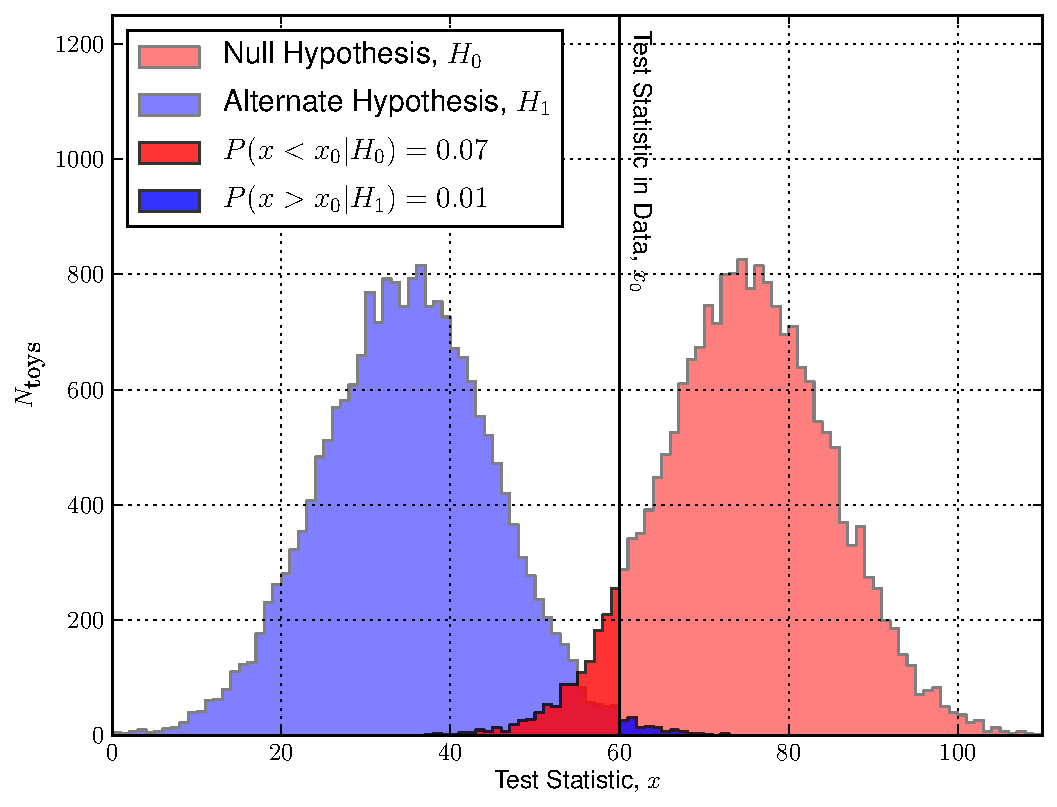
\includegraphics[width=0.49\textwidth]{fig/cls1}}
\subfloat[]{\label{fig:inter_cls_explain2}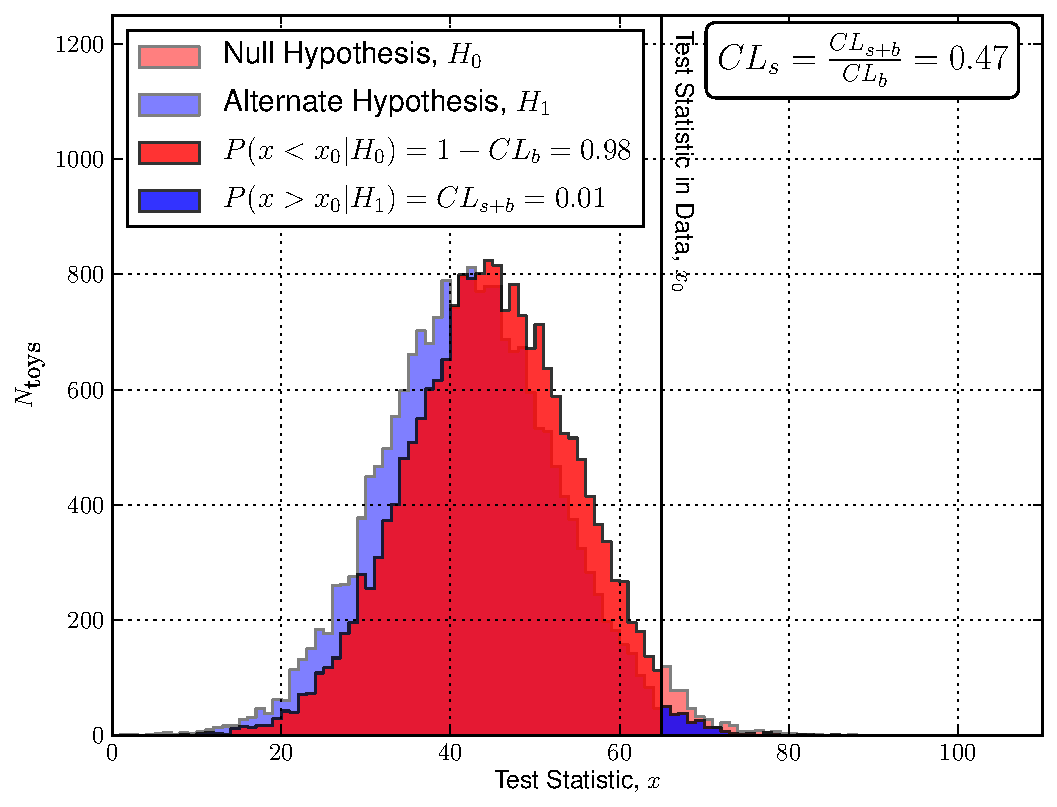
\includegraphics[width=0.49\textwidth]{fig/cls2}}
\caption[]{}
\label{fig:inter_cls_explain}
\end{figure}

\subsection{The \CLs Method}
One deficiency of the above method is that often the two hypotheses will not be
so well separated. This situation is shown in
Figure~\ref{fig:inter_cls_explain2}. In this case, the p-value for the alternate
hypothesis is small and so would result in an exclusion. This is undesirable
since the test statistic is clearly not sensitive enough to distinguish the two
hypotheses.

To address this problem, the \CLs hypothesis test may be used instead,
\begin{equation*}
\CLs = \frac{CL_{s+b}}{CL_{b}}
\end{equation*}
where, for the example shown in Figure~\ref{fig:inter_cls_explain2},
\begin{eqnarray*}
CL_{s+b} = P\left(x > x_0 | H_1\right)\\
CL_b = 1 - P\left(x < x_0 | H_0\right)
\end{eqnarray*}
where the null hypothesis now represents a background-only ($b$) scenario, and
the alternate, signal-plus-background ($s+b$). Using the \CLs to test the
alternate hypothesis, instead of a p-value, penalises cases where the test
statistic provides little sensitivity - since $CL_b$ will be large. For a 95\%
exclusion, $\CLs < 0.05$ is required, as before. \CLs may also be used to derive
an upper limit on some parameter by scanning through different values of the
parameter of interest in order to obtain a 95\% upper limit. This is known as
``hypothesis test inversion''.

Several additional details are relevant to the discussion here. Firstly, the toy
experiments used to generate distributions of the test statistic redice values
of the nuisance parameters around their expected values. The test statistic used
is the one-sided profile likelihood \cite{cl_computation, modified_frequentist, atlas_cms_higgs}.



\section{Modelling the Single Lepton Analysis}
As described in the previous section, the core component of many statistical
interpretations is the construction of an appopriate likelihood function. The
likelihood must model all statistical and systematic effects and is thus highly
dependent on the experiment. The situation is considerably complicated when
shape information is included, for which relevant bin-to-bin correlations must
be included.

\subsection{Notation}
It will be helpful to define some notation. In the following, a subscript index
is assumed to run over the binned variable in the analysis
(i.e. \STlep). All nuisance parameters are written as $\nu^{(i)}$ where the
superscript index is taken to run over some set of systematics
(e.g. $\nu^{\textrm{jes}}$ might represent a jet energy scale
uncertainty). Certain variables $x$ are known to have a functional dependence on a
given nuisance parameter and are written $x(\nu)$. The nominal value of this
variable, being that which is measured in \ac{MC} or in real data is denoted
$\bar{x}$.

\subsection{The Likelihood Function}
In constructing the likelihood, we start by writing down the number of events
expected for each bin (assigned the index $i=0,1,2...$):
\begin{equation}
\NExpi = \NSigi(\mu, \nu^{(j)}) +
\NBkgi(\nu^{(k)}) \\
\end{equation}
where \NSigi is the expected signal yield for a chosen
signal model and \NBkgi is the data-driven background
prediction. As can be seen, the signal yield is a function of the \ac{poi} (the
signal strength) and some number of nuisance parameters where the index $j$
will run over a set of systematics relevant to the signal yield. Ignoring
signal contamination effects (which will be discussed later), the bacground
yield depends only on the nuisance parameters $\nu^{(k)}$ where $k$ is taken to run
over the set of systematics relevant to the bacground prediction.

Without giving an explicit functional form for the signal yield and background
prediction, the form of the likelihood function may be constructed. The
likelihood must include:
\begin{enumerate}
\item Statistical terms representing the likelihood of observing the given
  number of events given a certain expectation for the signal and background
  yields.
\item Terms providing prior constraints on the various nuisance
  parameters. Certain uncertainties are statistical in nature and thus,
  indepdent nuisance parameters are assigned per bin along with a corresponding
  prior pdf. In other cases, the underlying systematic variation is considered
  to have a 100\% correlated effect across the bins. In these cases, a single
  nuisance parameter and prior pdf is assigned.
\end{enumerate}

The form of the likelihood is as follows,
\begin{equation}
\mathcal{L} = \prod_i \Poisson(\NExpi ; \NObsi)
\prod_{\alpha \in \Theta}  X_\alpha(\nu^{(\alpha)})
\end{equation}
where
\begin{itemize}
\item $\mathcal{P}(\mu;x)$ denotes a Poisson distribution with mean $\mu$ and value
$x$
\item The $X_\alpha(\nu^{(\alpha)})$ represent some prior pdf associated with
  each systematic $\alpha$.
\end{itemize}

\subsection{The Signal Yield}
The signal yield per bin is constructed as follows
\begin{equation}
\NSigi = \mu \times \epsilon_i(\nu^{(\alpha)}) \times \sigma \times L \times \nu^{\textrm{lumi}}
\end{equation}

with
\begin{itemize}
\item $\epsilon_i(\nu^{(\alpha)})$ is the efficiency of the $i$th bin assumed to be
  dependent on a set of nuisance parameters $\nu^{(\alpha)}$.
\item $\sigma$ the cross-section of the signal model being considered,
\item $L$ the integrated luminosity,
\item $\nu^{\textrm{lumi}}$ the nuisance parameter associated with uncertainty in the
estimate of the integrated luminosity.
\end{itemize}

\subsection{Background Prediction}
The background prediction per bin is then written as
\begin{equation}
\NBkgi = \RCSi(\nu_i^{(\alpha)}, \nu^{(\beta)}) \times \NControli(\nu_i^{(\gamma)})
\end{equation}
where
\begin{itemize}
\item \RCSi is the translation ratio as defined in Section TODO,
\item The nuisance parameters $\nu_i^{(\alpha)}$ and $\nu_i^{\gamma}$ represent
  statistical uncertainties uncorrelated between the bins.
\item The nuisance parameters $\nu_i^{(\beta)}$ represent systematic
  uncertainties assumed to be 100\% correlated across the bins.
\item \NControli the observed number of events in the control region
($L_P > 0.3$)
\end{itemize}

\subsection{Parameterising Systematics}
In reality, it is almost always impossible to obtain a full functional form for
a variable $x$ (e.g. \RCSi, \NControli) in terms of a set of nuisance parameters
$\nu^{(\alpha)}$. Writing the Taylor expansion of $x(\nu^{(\alpha)})$ for two terms to
second order,
\begin{align*}
 x(\nu^{(A)}, \nu^{(B)})\bigg|_{\substack{\nu^{(A)} = a\\ \nu^{(B)} = b}} \approx
x(a,b) +
(\nu^{(A)} - a)\left.\frac{\partial x}{\partial\nu^{(A)}}\right|_{\nu^{(A)}=a} +
(\nu^{(B)} - b)\left.\frac{\partial x}{\partial\nu^{(B)}}\right|_{\nu^{(B)}=b} +\\
\frac{1}{2!}\left[
(\nu^{(A)} - a)^2 \frac{\partial^2 x}{\partial \left(\nu^{(A)}\right)^2}
+ (\nu^{(B)} - b)^2 \frac{\partial^2 x}{\partial \left(\nu^{(B)}\right)^2}
+ 2(\nu^{(A)} - a)(\nu^{(B)} - b)\frac{\partial^2 x}{\partial
  \nu^{(A)}\partial\nu^{(B)}}
\right]
\end{align*}
Assuming the expansion is performed with respect to the mean of x, $\bar{x}$,
the values of $a$ and $b$ are seen to be the mean values of the corresponding nuisance
parameters. For small deviations from the mean,
\begin{equation}
 (\nu^{(A)} - a) \sim (\nu^{(B)} - b) \sim \epsilon \sim 0
\end{equation}
and ignoring terms $O(\epsilon^2)$

\begin{equation}
x(\nu^{(A)}, \nu^{(B)}) \approx \bar{x} +
(\nu^{(A)} - a)\left.\frac{\partial x}{\partial\nu^{(A)}}\right|_{\nu^{(A)}=a} +
(\nu^{(B)} - b)\left.\frac{\partial x}{\partial\nu^{(B)}}\right|_{\nu^{(B)}=b}
\label{eqn:stats:taylor}
\end{equation}
Since the derivatives in Equation~\ref{eqn:stats:taylor} will in practice be
derived from some finite variation of the underlying quantity associated with
each nuisance parameter, the infinitessimal derivatives must be replaced by
finite changes. It is also sensible to set $a=b=0$.
\begin{equation}
x(\nu^{(A)}, \nu^{(B)}) \approx \bar{x} +
\nu^{(A)}\frac{\Delta x}{\Delta\nu^{(A)}} +
\nu^{(B)}\frac{\Delta x}{\Delta\nu^{(B)}}
\label{eqn:stats:taylor2}
\end{equation}
Since the value of $x$ is often associated with a physical quantity such as an
efficiency or an event yield, it is desirable to constrain it to positive
values. This can be achieved providing the range of each nuisance parameter is
set such that
\begin{equation}
\nu^{(\alpha)}\times\frac{\Delta x}{\Delta \nu^{(\alpha)}} < \bar{x}
\end{equation}

The previous derivation can be simply extended two $N > 2$ nuisance
parameters. Generalising and rewriting Equation~\ref{eqn:stats:taylor2},
\begin{eqnarray*}
x(\nu^{(A)}, \nu^{(B)}, \ldots) &\approx& \bar{x} +
\nu^{(A)}\frac{\Delta x}{\Delta\nu^{(A)}} +
\nu^{(B)}\frac{\Delta x}{\Delta\nu^{(B)}} + \ldots \\
&\approx& \frac{1}{\bar{x}^{N-1}} \left\{ \bar{x}^N +
\bar{x}^{N-1} \nu^{(A)}\frac{\Delta x}{\Delta\nu^{(A)}} +
\bar{x}^{N-1} \nu^{(B)}\frac{\Delta x}{\Delta\nu^{(B)}} + \ldots \right\}
\end{eqnarray*}
Trying to rewrite as a product,
\begin{eqnarray*}
\prod_{j=A, B, \ldots} \left(\bar{x} + \frac{\Delta x}{\Delta\nu^{(\alpha)}}\right) &=&
\bar{x}^N + \bar{x}^{N-1} \sum_{j=A, B, \ldots} \nu^{(\alpha)}\frac{\Delta x}{\Delta \nu^{(\alpha)}} \\
&&+ \bar{x}^{N-2}\sum_{j=A, B, \ldots} \sum_{k=A, B, \ldots} \nu^{(\alpha)}\nu^{(\beta)}\frac{\Delta x}{\Delta
  \nu^{(\alpha)}}\frac{\Delta x}{\Delta \nu^{(\beta)}} \\
&&+ \ldots +O(\nu^N)
\end{eqnarray*}
Ignoring terms greater than $O(\nu^2)$,
\begin{eqnarray*}
\prod_{j=A, B, \ldots} \left(\bar{x} + \frac{\Delta x}{\Delta\nu^{(\alpha)}}\right) &\approx&
\bar{x}^N + \bar{x}^{N-1} \sum_{j=A, B, \ldots} \nu^{(\alpha)}\frac{\Delta x}{\Delta
  \nu^{(\alpha)}} \\
&\approx& \bar{x}^{N-1} x(\nu^{(A)}, \nu^{(B)}, \ldots)
\end{eqnarray*}
and therefore
\begin{equation}
x(\nu^{(A)}, \nu^{(B)}, \ldots) \approx \frac{1}{\bar{x}^{N-1}} \prod_{j = A, B,
  \ldots} \left(\bar{x} + \frac{\Delta x}{\Delta\nu^{(\alpha)}}\right) \approx
\bar{x} \prod_{j = A, B,
  \ldots} \frac{1}{\bar{x}}\left(\bar{x} + \frac{\Delta x}{\Delta\nu^{(\alpha)}}\right)
\label{eqn:stats:systderiv}
\end{equation}

Using Equation~\ref{eqn:stats:systderiv}, the signal yield can be rewritten as follows
\begin{equation}
\NSigi = \mu \times \bar{\epsilon}_i \times \prod_{j}\left(\frac{\bar{\epsilon}_i
    + \nu^{(\alpha)}\frac{\Delta\epsilon_i}{\Delta\nu^{(\alpha)}}}{\bar{\epsilon}_i}\right) \sigma \times L \times \nu^{\textrm{lumi}}
\end{equation}
and the background prediction
\begin{equation}
\NBkgi = \RbarCS_i \times \prod_{j}\left( \frac{\RbarCS_i
    + \nu^{(\alpha)}\frac{\Delta\RCSi}{\Delta\nu^{(\alpha)}}}{\RbarCS_i}\right)
\times \NbarControl_i \times \prod_{k}\left( \frac{\NbarControl_i
    + \nu^{(\alpha)}\frac{\Delta\NControli}{\Delta\nu^{(\beta)}}}{\NbarControl_i}\right)
\end{equation}

\subsection{Nuisance Parameters}
The nuisance parameters incorporated in the model described thus far are of two
types.
\begin{enumerate}
\item Statistical uncertainties assumed to be uncorrelated across analysis
  bins. This includes uncertainties arising from limited generator statistics,
  limited data in the control region and signal contamination in the control
  region.
\item Systematic uncertainties arising from detector artefacts or theoretical
  uncertainties such as jet energy scale, standard model cross-sections and
  integrated luminosity measurement.
\end{enumerate}
For uncertainties of the first kind, independent nuisance paramters must be
included for each analysis bin. For uncertainties of the second kind, a
single nuisance parameter will be included for all bins. This achieves the
desired correlation. A full list of the nuisance parameters used is shown in
Table~\ref{tbl:systematic_parameters}.

\ctable[
cap=Nuisance parameters included in the single lepton likelihood function,
caption=Summary of nuisance parameters included in the single lepton likelihood function.,
mincapwidth=0.5\textwidth,
label=tbl:inter_systematic_parameters,
pos=h,
doinside=\scriptsize
]{lccccc}{
\tnote[a]{Muon channel only}
\tnote[b]{Electron channel only}

\tnote[c]{In the electron channel, the use of \ac{MC} templates in the QCD
  background estimate introduces a dependence on the \ac{JES}. Whilst the
  ability to include these correlations was added to the statistics package, it
  was not used in the results shown.}

}{\FL
Uncertainty                        & Correlated & \NSigi     & \RCSi      & \NControli & Nuisance Parameters\ML
%
Luminosity                         & \checkmark & \checkmark &            &            & $\nu^{\textrm{lumi}}$\NN
\acf{JES}                          & \checkmark & \checkmark & \checkmark & \tmark[c]  & $\nu^{\textrm{jes}}$\NN
\MET Resolution                    & \checkmark & \checkmark & \checkmark & \tmark[c]  & $\nu^{\textrm{metres}}$\NN
\PW/\Ptop\APtop Ratio              & \checkmark &            & \checkmark &            & $\nu^{W\Ptop\APtop}$\NN
\PW Polarisation                   & \checkmark &            & \checkmark &            & $\nu^{\textrm{\PW pol}}$\NN
Muon Momentum Scale\tmark[a]       & \checkmark &            & \checkmark &            & $\nu^{\textrm{lep}}$\NN
Limited \ac{MC} Statistics         &            &            & \checkmark &            & $\nu^{\textrm{MC}}_i$\NN
Limited Data Statistics            &            &            &            & \checkmark & $\nu^{\textrm{data}}_i$\NN
Signal Contamination               &            &            &            & \checkmark & $\nu^{\textrm{sig cont}}_i$\NN
\ac{PDF} Uncertainties             & \checkmark & \checkmark &            &            & $\nu^{\textrm{pdf}}_i$\NN
QCD Background Prediction\tmark[b] &            &            &            & \checkmark & $\nu^{\textrm{qcd}}_i$\LL
}

\subsection{Signal Contamination}
It can be seen in Figure~TODO that the region \LPcontrol may have a substantial
component of \ac{SUSY} events depending on the particular model under
consideration. Signal contamination increases \NControl leading to an
overprediction of \NBkg. To account for this, the \NBkgi term is modifed to
reflect the assumption that some fraction of the yield \NControli will be
due to \ac{SUSY} contamination. Rewriting,

\begin{equation}
\NBkgi(\mu, \nu^{(\alpha)}) = \RbarCS_i \times \prod_{j}\left( \frac{\RbarCS_i
    + \nu^{(\alpha)}\frac{\Delta\RCSi}{\Delta\nu^{(\alpha)}}}{\RbarCS_i}\right)
\times \NbarControl_i \times f^{\textrm{SM}}_i(\mu) \times \prod_{k}\left( \frac{\NbarControl_i
    +
    \nu^{(\alpha)}\frac{\Delta\NControli}{\Delta\nu^{(\beta)}}}{\NbarControl_i}\right)
\label{eqn:bgprediction}
\end{equation}
where $f^{\textrm{SM}}_i$ represents the fraction of \NControli expected to be
\ac{SM} events given the current signal hypothesis i.e.
\begin{equation}
f^{\textrm{SM}}_i(\mu) = \frac{\NSMi}{\NSMi + \NSUSYi(\mu)}
\end{equation}
The expected number of \ac{SUSY} events $\NSUSYi =
\mu\times\epsilon^{\textrm{control}}_i\times\sigma\times L$ where
$\epsilon^{\textrm{control}}_i$ is the efficiency calculated for \ac{SUSY}
events entering the \LPcontrol control region. To reflect these constraints, we
setup an appropriate prior distribution
\begin{equation}
X(\nu^{\textrm{SM}}) = \Gauss \left( \frac{\NSMi}{\NSMi + \mu\times\epsilon_i^{\textrm{control}}\times\sigma\times L}
; \nu^{\textrm{SM}} \right)
\end{equation}
and $f^{\textrm{SM}}_i \equiv \nu^{\textrm{SM}}_i$. Calculating the expected value of the nuisance parameter,
\begin{eqnarray}
<f^{\textrm{SM}}_i> &=& \frac{\NSMi}{\NSMi + \mu\NSUSYi} \\
                   &=& \frac{1}{1 + \mu\frac{\NSUSYi}{\NSMi}}
\label{eqn:fSMideal}
\end{eqnarray}
Technical problems associated with adding a functional dependence on the
\ac{poi} $\mu$ to the mean of the prior distribution necessitated a slightly
altered formulation. As will be shown, this formulation is approximately
equivalent given certain assumptions about the range of $\mu$ and the degree of
signal contamination. The prior distribution included in \likelihood is
rewritten as
\begin{equation}
X(\nu^{\textrm{SM}}_i) = \Gauss \left( \frac{\NSMi}{\NSMi + \epsilon_i^{\textrm{control}}\times\sigma\times L}
; \nu^{\textrm{SM}}_i \right)
\end{equation}
The term included in the background prediction (\ref{eqn:bgprediction}) is modified to
\begin{equation}
f^{\textrm{SM}}_i = 1 - \mu \times \left(1- \nu^{\textrm{SM}}_i\right)
\end{equation}
It can be seen that for $\mu=0$, $f^{\textrm{SM}}_i=1$ and for $\mu=1$,
$f^{\textrm{SM}}_i=\nu^{\textrm{SM}}_i$ as required. It will now be shown that
for a suitable range of $\mu$ and for small values of $\NSUSYi/\NControli$, the
expectation value of $f^{\textrm{SM}}_i$ will be equivalent to
Equation~\ref{eqn:fSMideal}.
\begin{eqnarray*}
<f^{\textrm{SM}}_i> &=& 1 - \mu \times \left(1-<\nu^{\textrm{SM}}>\right) \\
                  &=& 1 - \mu  + \mu\frac{\NSMi}{\NSMi + \NSUSYi} \\
                  &=& \frac{(1-\mu)\left(\NSMi + \NSUSYi\right) + \mu\NSMi}{\NSMi + \NSUSYi} \\
                  &=& \frac{\NSMi + (1 - \mu)\NSUSYi}{\NSMi + \NSUSYi} \\
                  &=& \frac{\NSMi \left( 1 + (1-\mu)\frac{\NSUSYi}{\NSMi}\right)}{\NSMi + \NSUSYi} \\
                  &=& \frac{\NSMi}{\left(\NSMi +\NSUSYi\right)\left( 1 + (1 - \mu)\frac{\NSUSYi}{\NSMi}\right)^{-1}} \\
                  &\approx& \frac{\NSMi}{\left(\NSMi +\NSUSYi\right)\left( 1 - (1-\mu)\frac{\NSUSYi}{\NSMi}\right)} \\
                  &=& \frac{\NSMi}{\NSMi + \mu\NSUSYi - (1-\mu)\frac{\NSUSYi^2}{\NSMi}}\\
                  &=& \frac{1}{1 + \mu\frac{\NSUSYi}{\NSMi} - (1-\mu)\left(\frac{\NSUSYi}{\NSMi}\right)^2} \\
                  &\approx& \frac{1}{1 + \mu\frac{\NSUSYi}{\NSMi}}
\end{eqnarray*}

\subsection{Uncertainties on \NControli}
The dominant systematic uncertainty relating to the \LPcontrol region yield
arises from the limited statistics of the sample. This is especially true at
high \STlep. Accordingly, a nuisance parameter is added to the likelihood and
assigned a Gaussian prior with a width derived assuming a Poisson error on the
\NControli yield.

An additional complication arises in the case of the electron channel where the
\LPcontrol region has a non-negligible component of \ac{QCD} multijet
events. These are unreliably modelled by event generators and thus not included
in the calculation of \RCSi. This additional contribution to \NControli would
again lead to an overprediction of the background. To correct this, an
additional factor is included in Equation~\ref{eqn:bgprediction},
$f^{\textrm{ewk}}_i$ derived from the results of the \ac{QCD} fit detailed in
Section~TODO. The error derived from the fit procedure is modelled as a
Gaussian prior on an additional nuisance parameter $\nu^{\textrm{QCD}}_i$. It
has been assumed, and confirmed by the results of the fit in data that the
region \LPsignal is \ac{QCD} free.

The uncertainty included via the prior distribution of $\nu^{\textrm{QCD}}$ was
the quadrature sum of the statistical error from the fitting procedure and an
uncertainty accounting for the limited generator statistics used to construct
the fit templates. Additional errors coming from jet energy scale uncertainty
and missing energy resolution were found to be small. Proper inclusion of these
into the likelihood would need to ensure correlation with the nuisance
parameters representing these uncertainties. The relevant terms were setup but
not included in the final calculations. The contribution is seen to be small and
unnecessary complication of the likelihood function tends to increase the
processing time, especially when running a large number of toy experiments.

\begin{figure}
\centering
\subfloat[]{\label{fig:inter_pl_80_400_syst}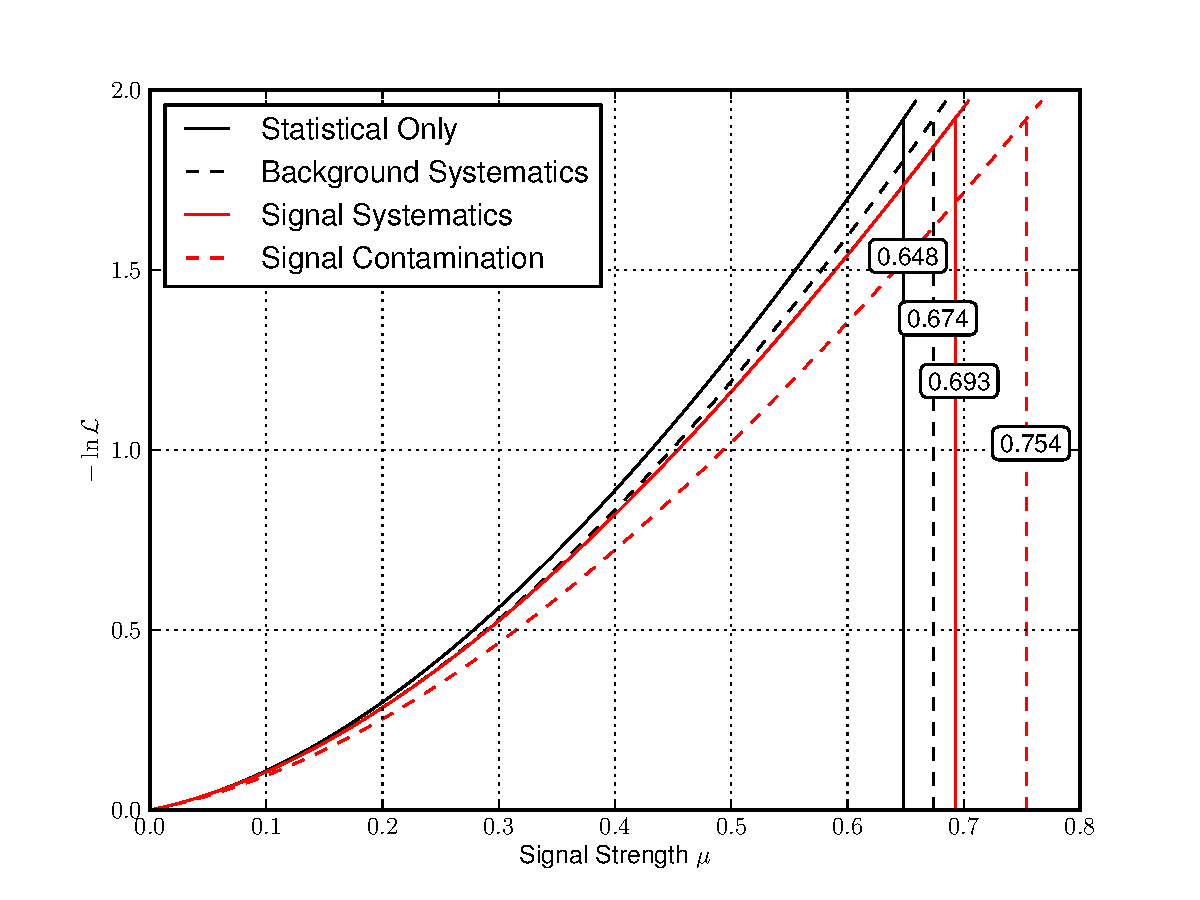
\includegraphics[width=0.47\textwidth]{fig/pl_systematics_80_400}}\quad
\subfloat[]{\label{fig:inter_pl_80_400_muon}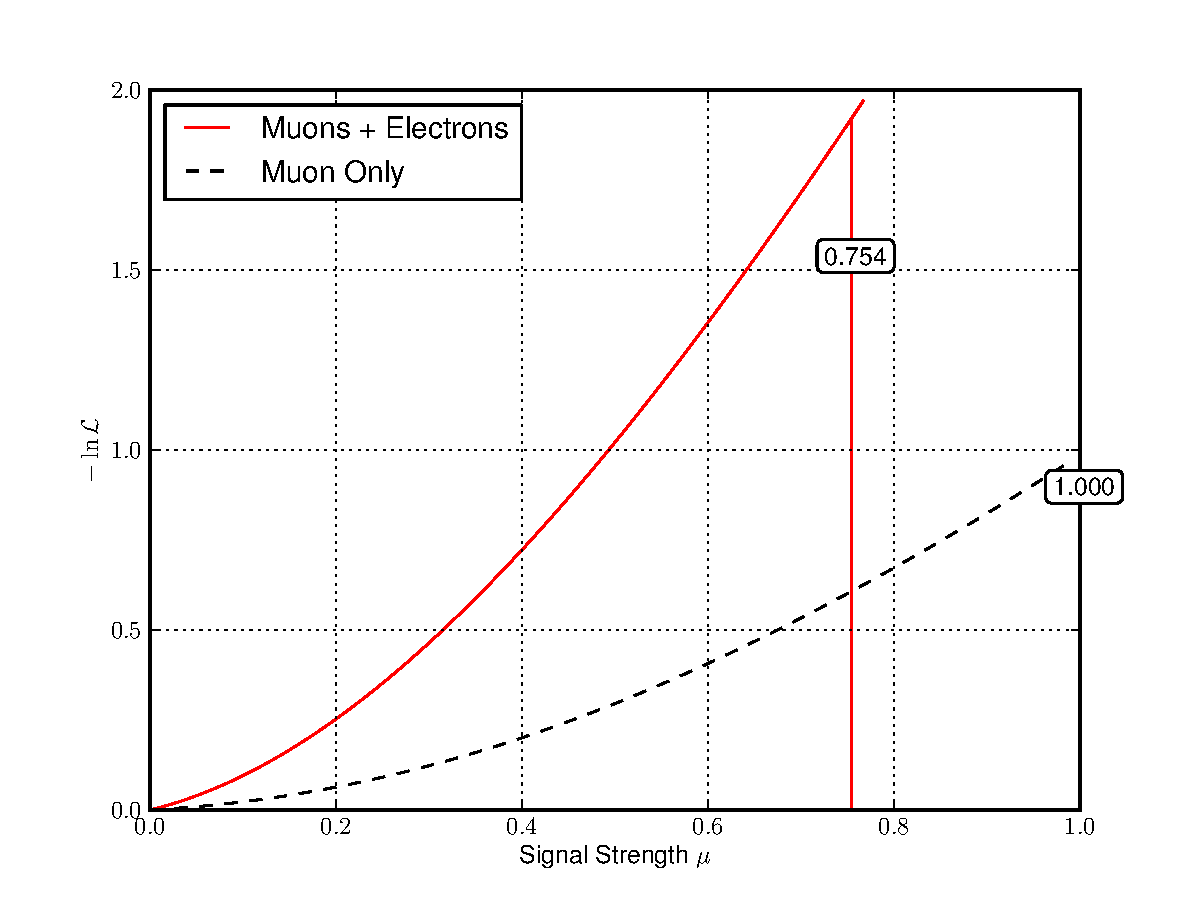
\includegraphics[width=0.47\textwidth]{fig/pl_muon_80_400}}
\caption[]{}
\label{fig:inter_pl}
\end{figure}

\begin{figure}
\centering
\subfloat[Statistical Uncertainties Only]{
  \label{fig:inter_cls_80_400_syst}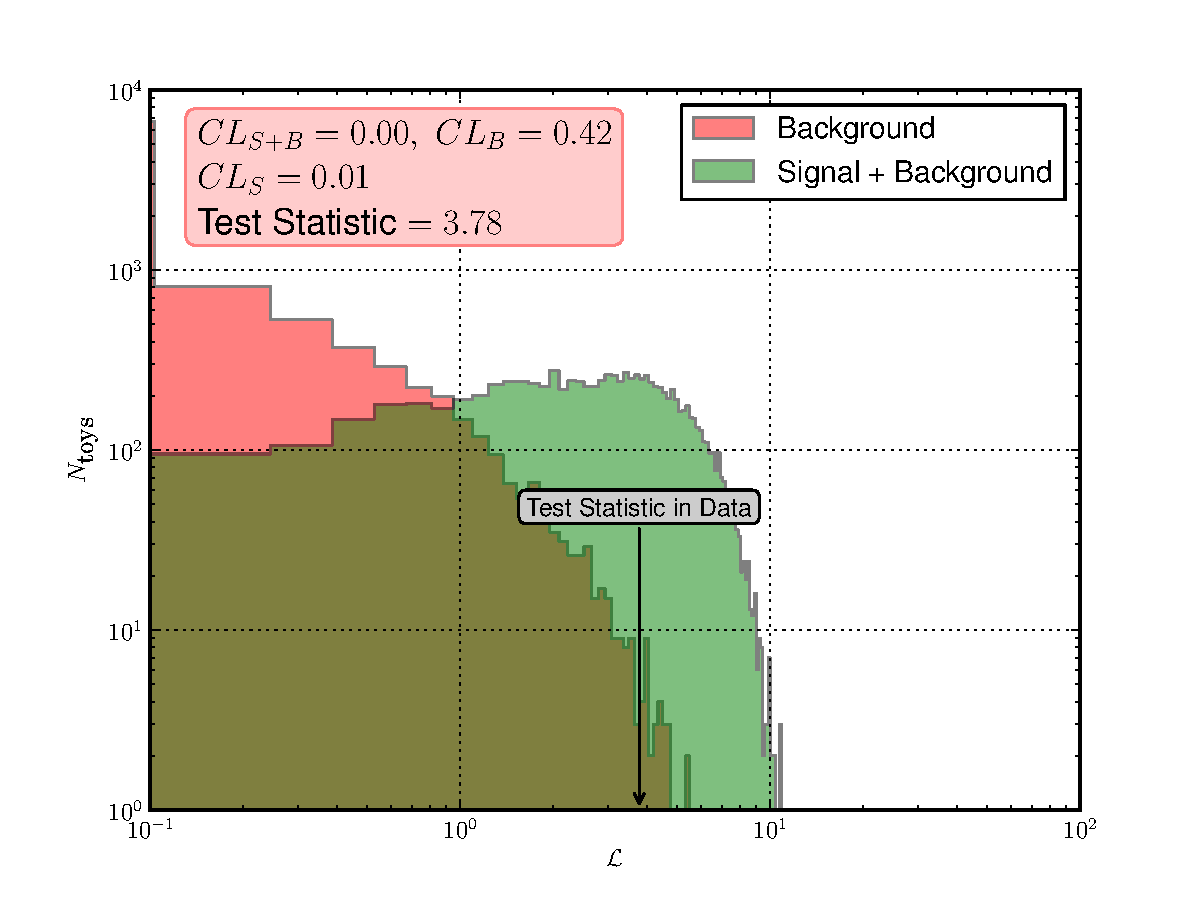
\includegraphics[width=0.47\textwidth]{fig/exp_muon_electron_80_400_bgsysts_no_sigsysts_no_sigcon_no}}\quad
\subfloat[Background Systematics]{
  \label{fig:inter_cls_80_400_muon}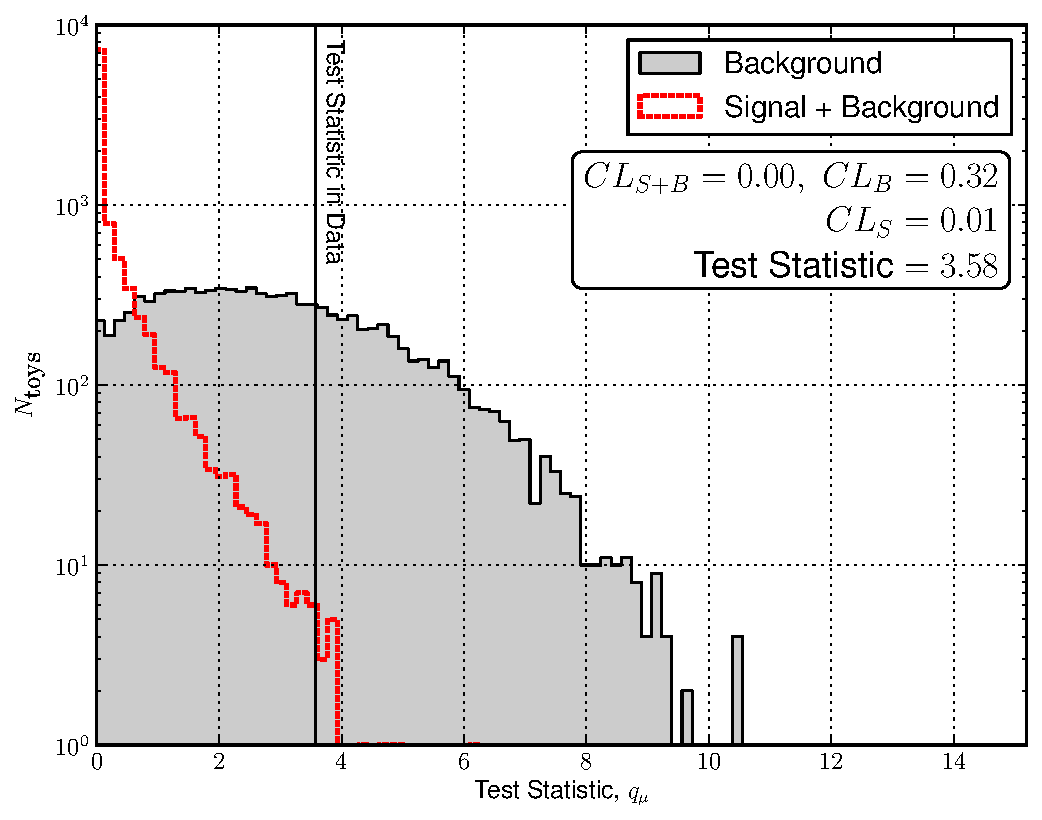
\includegraphics[width=0.47\textwidth]{fig/exp_muon_electron_80_400_bgsysts_yes_sigsysts_no_sigcon_no}}\\
\subfloat[Signal Systematics]{
  \label{fig:inter_cls_80_400_syst}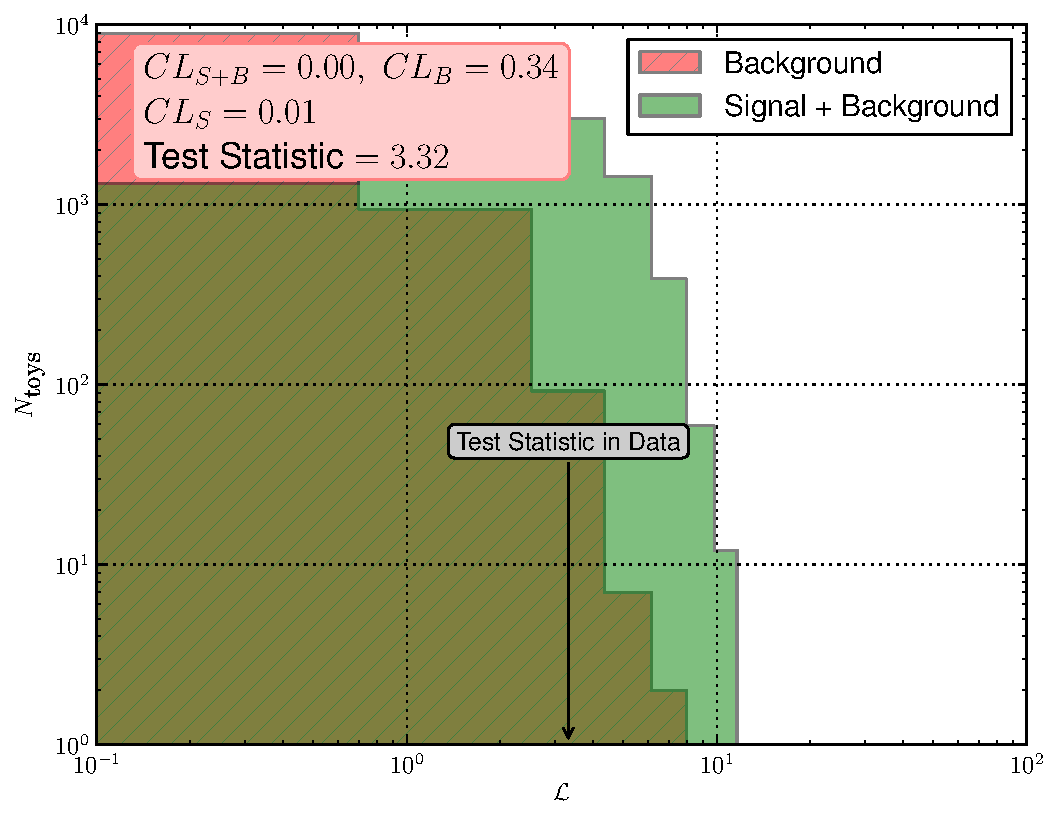
\includegraphics[width=0.47\textwidth]{fig/exp_muon_electron_80_400_bgsysts_yes_sigsysts_yes_sigcon_no}}\quad
\subfloat[Signal Contamination]{
  \label{fig:inter_cls_80_400_muon}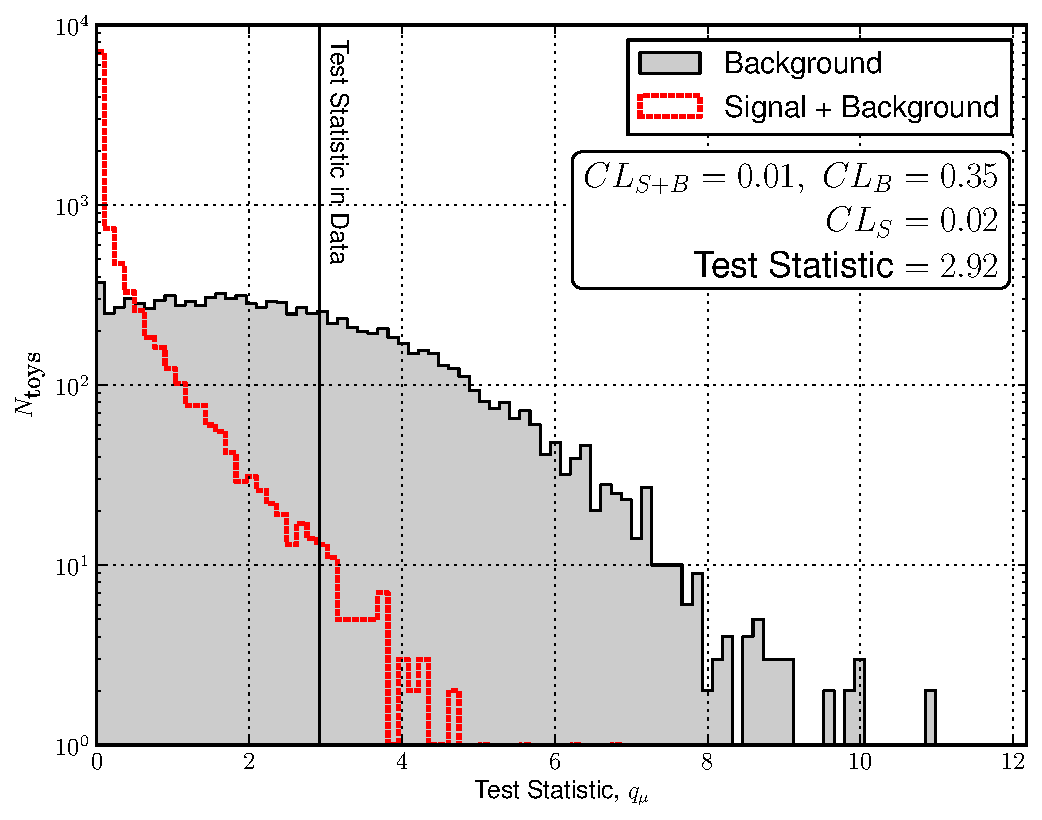
\includegraphics[width=0.47\textwidth]{fig/exp_muon_electron_80_400_bgsysts_yes_sigsysts_yes_sigcon_yes}}\\
\subfloat[Muon Channel Only]{
  \label{fig:inter_cls_80_400_muon}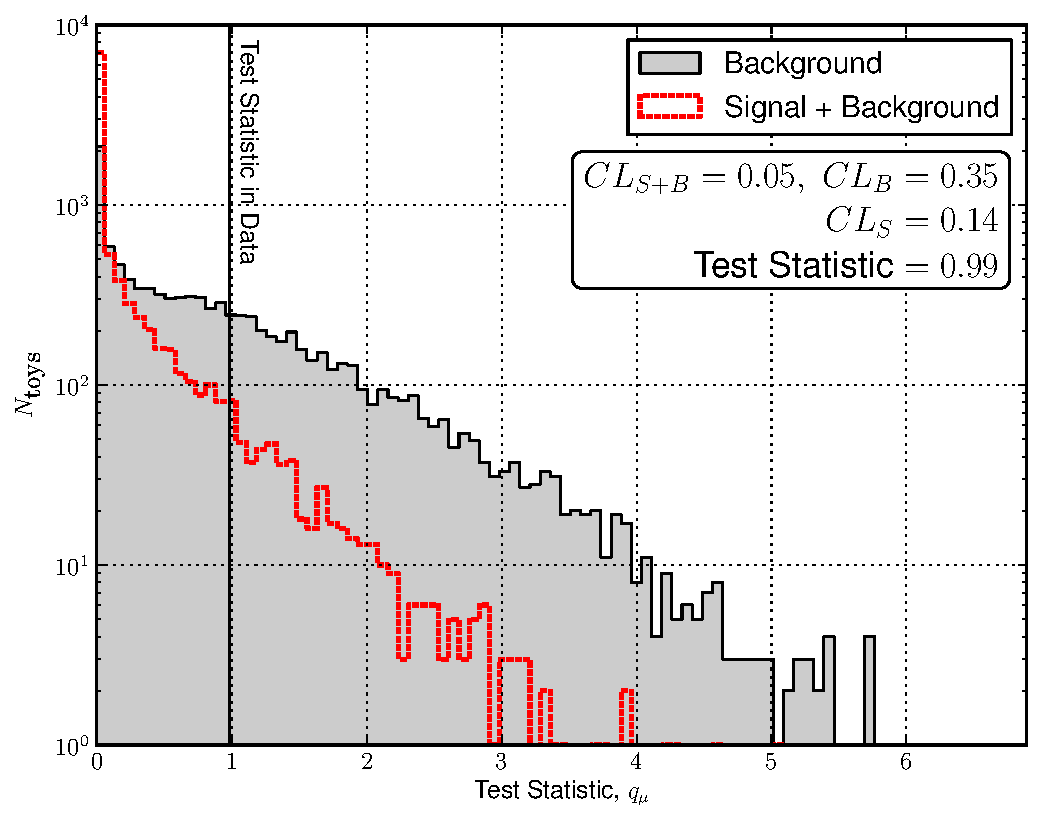
\includegraphics[width=0.47\textwidth]{fig/exp_muon_80_400_bgsysts_yes_sigsysts_yes_sigcon_yes}}
\caption[]{}
\label{fig:inter_cls}
\end{figure}

\section{Results}
The likelihood model is used to provide interpretation within the context of two
\ac{NP} models: \ac{mSUGRA} and the \ac{T2tt} simplified model described in
Section~TODO.

\subsection{\ac{mSUGRA}}
The efficiency per \STlep bin of the analysis selection as a function of the
\ac{mSUGRA} parameter space is shown in Figures~\ref{fig:inter_msugra_mu} and
\ref{fig:inter_msugra_el} for muons and electrons respectively. The ``holes'' in
the \ac{mSUGRA} sample are due to incomplete data samples at the time of
publication. The relation of the \STlep variable to the model parameters is
readily apparent.

\begin{figure}
\centering
\subfloat[]{\label{fig:inter_msugra_mu_eff250}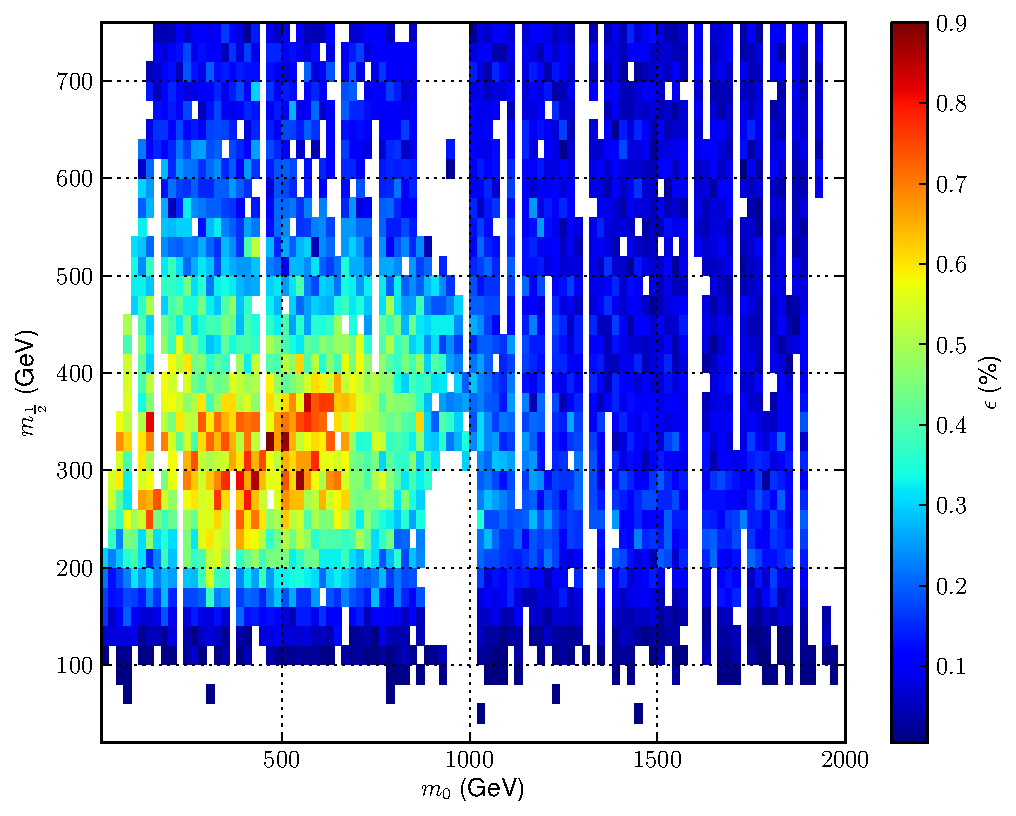
\includegraphics[width=0.49\textwidth]{fig/msugra_muons_eff_250}}
\subfloat[]{\label{fig:inter_msugra_mu_eff350}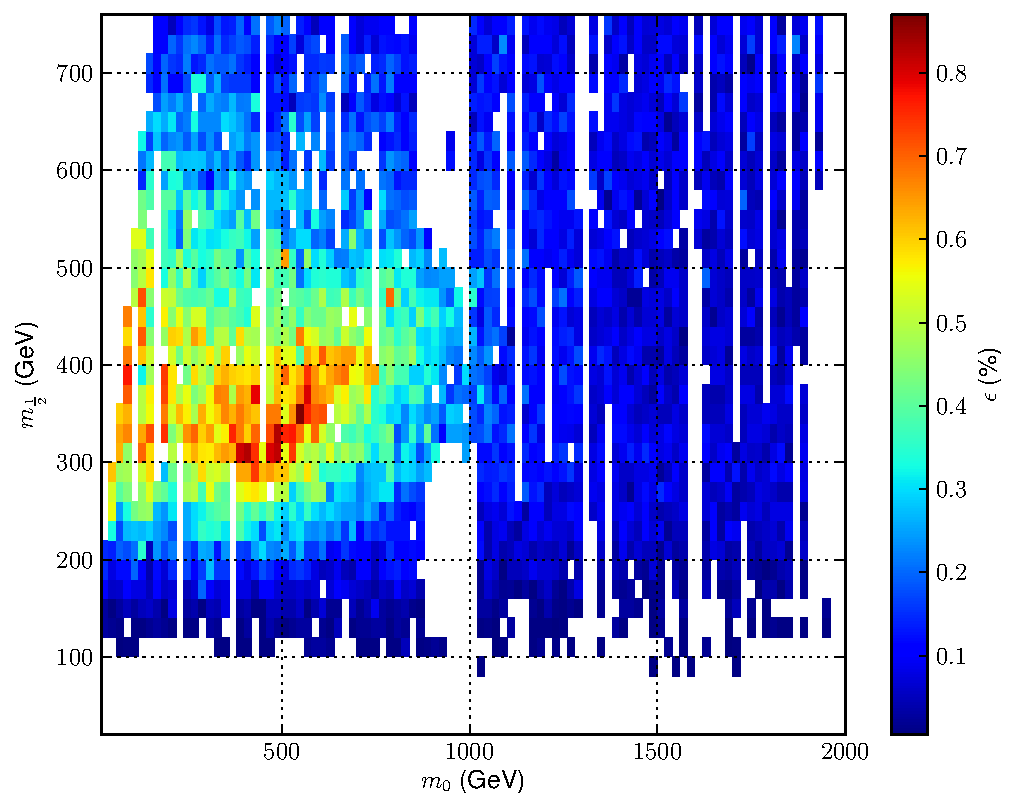
\includegraphics[width=0.49\textwidth]{fig/msugra_muons_eff_350}}\\
\subfloat[]{\label{fig:inter_msugra_mu_eff450}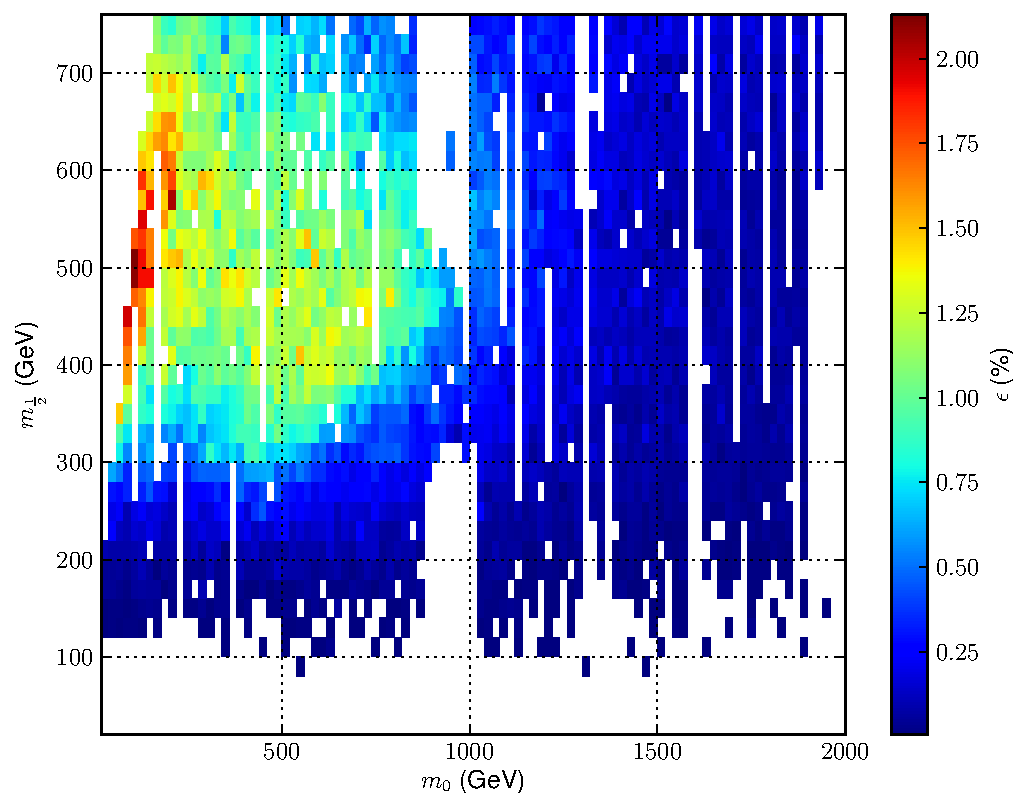
\includegraphics[width=0.49\textwidth]{fig/msugra_muons_eff_450}}
\subfloat[]{\label{fig:inter_msugra_mu_efftot}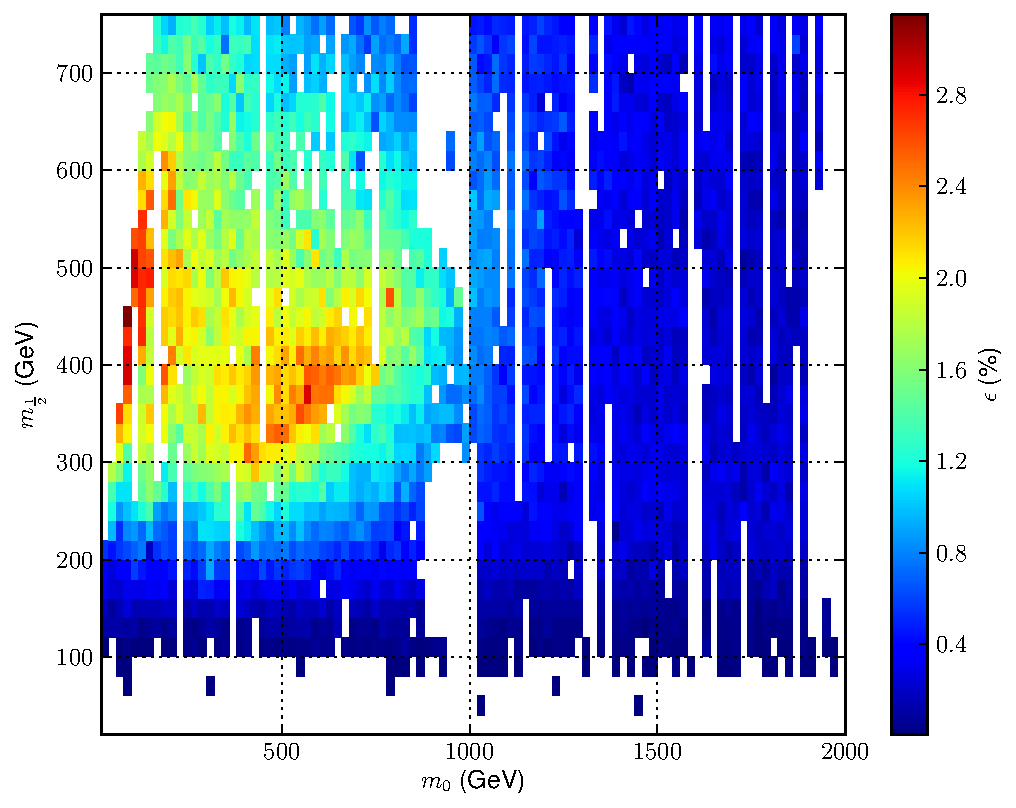
\includegraphics[width=0.49\textwidth]{fig/msugra_muons_eff_total}}
\caption[]{}
\label{fig:inter_msugra_mu}
\end{figure}

\begin{figure}
\centering
\subfloat[]{\label{fig:inter_msugra_el_eff250}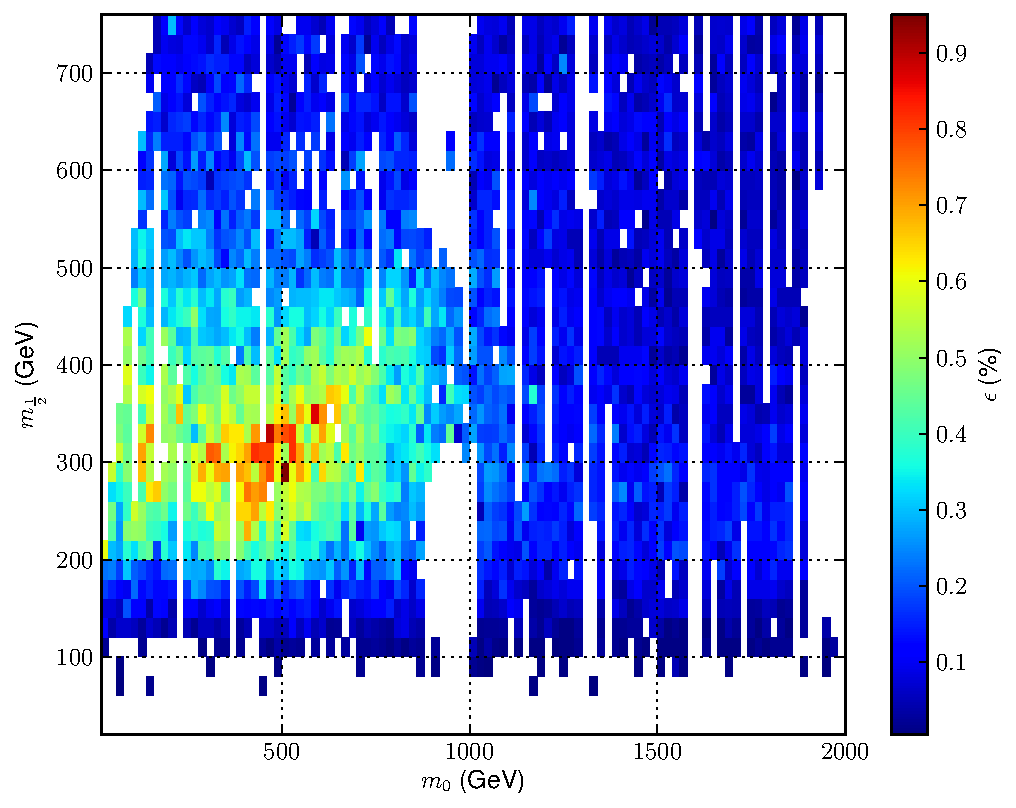
\includegraphics[width=0.49\textwidth]{fig/msugra_electrons_eff_250}}
\subfloat[]{\label{fig:inter_msugra_el_eff350}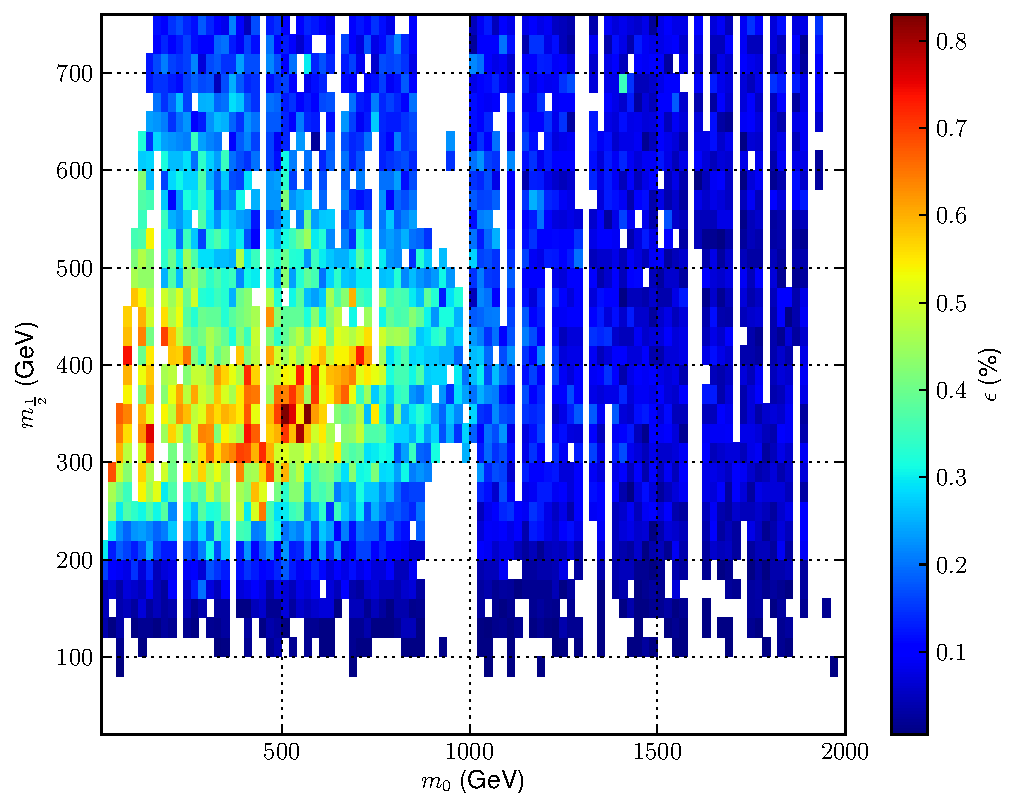
\includegraphics[width=0.49\textwidth]{fig/msugra_electrons_eff_350}}\\
\subfloat[]{\label{fig:inter_msugra_el_eff450}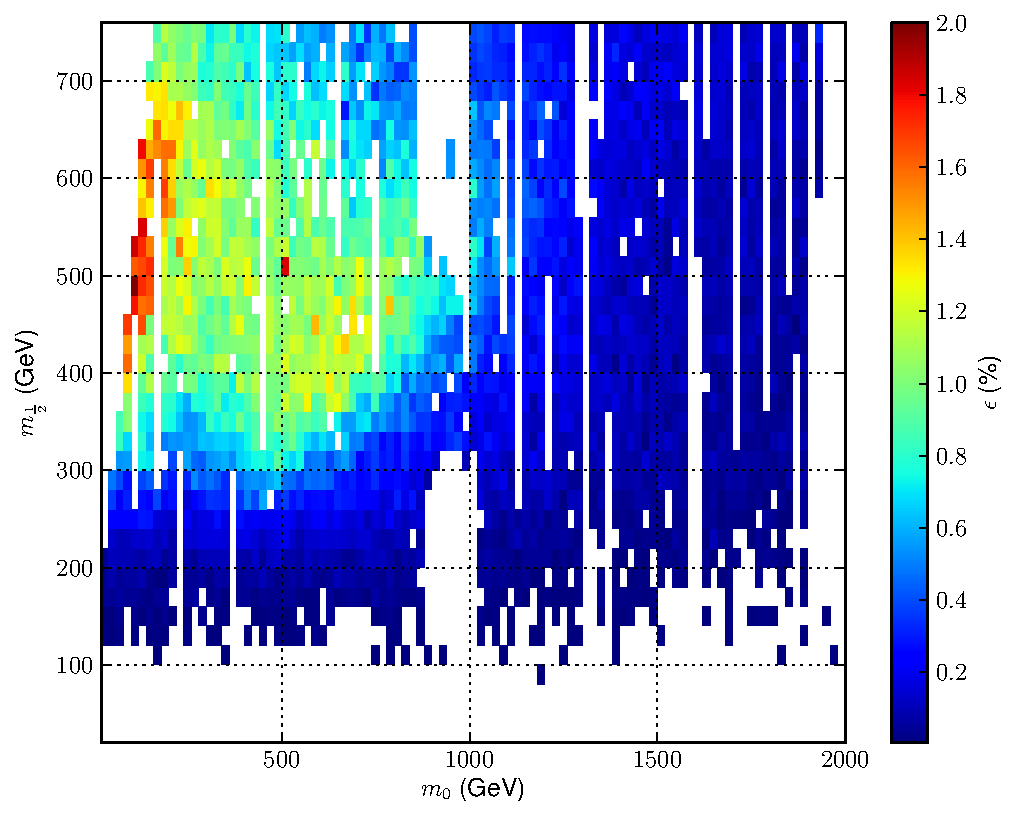
\includegraphics[width=0.49\textwidth]{fig/msugra_electrons_eff_450}}
\subfloat[]{\label{fig:inter_msugra_el_efftot}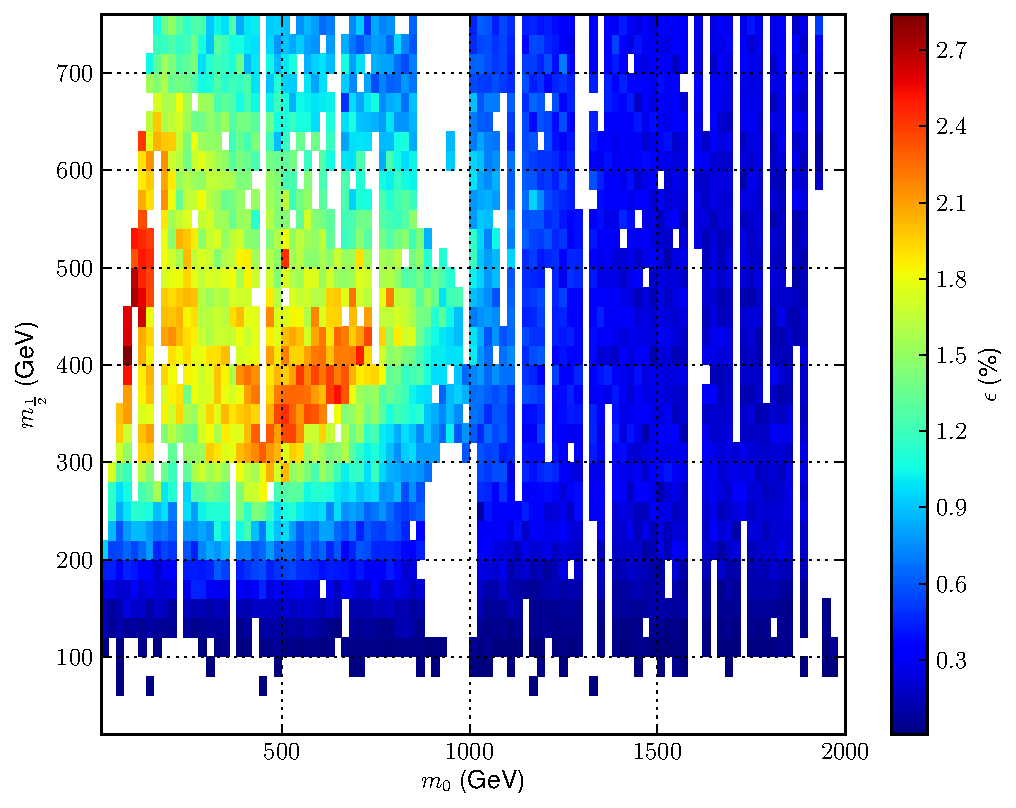
\includegraphics[width=0.49\textwidth]{fig/msugra_electrons_eff_total}}
\caption[]{}
\label{fig:inter_msugra_el}
\end{figure}

For consistency with other \ac{SUSY} searches at the \ac{LHC}, a limit has been
set using the \CLs method described in Section~\ref{sec:inter_cls}. Whilst
it is possible, to set an upper limit on the signal strength parameter, $\mu$,
this becomes highly computationally intensive. Instead, a simple exclusion was
produced assuming \ac{NLO} cross-sections. This is shown in
Figure~\ref{fig:inter_msugra_exclusion}.

\begin{figure}
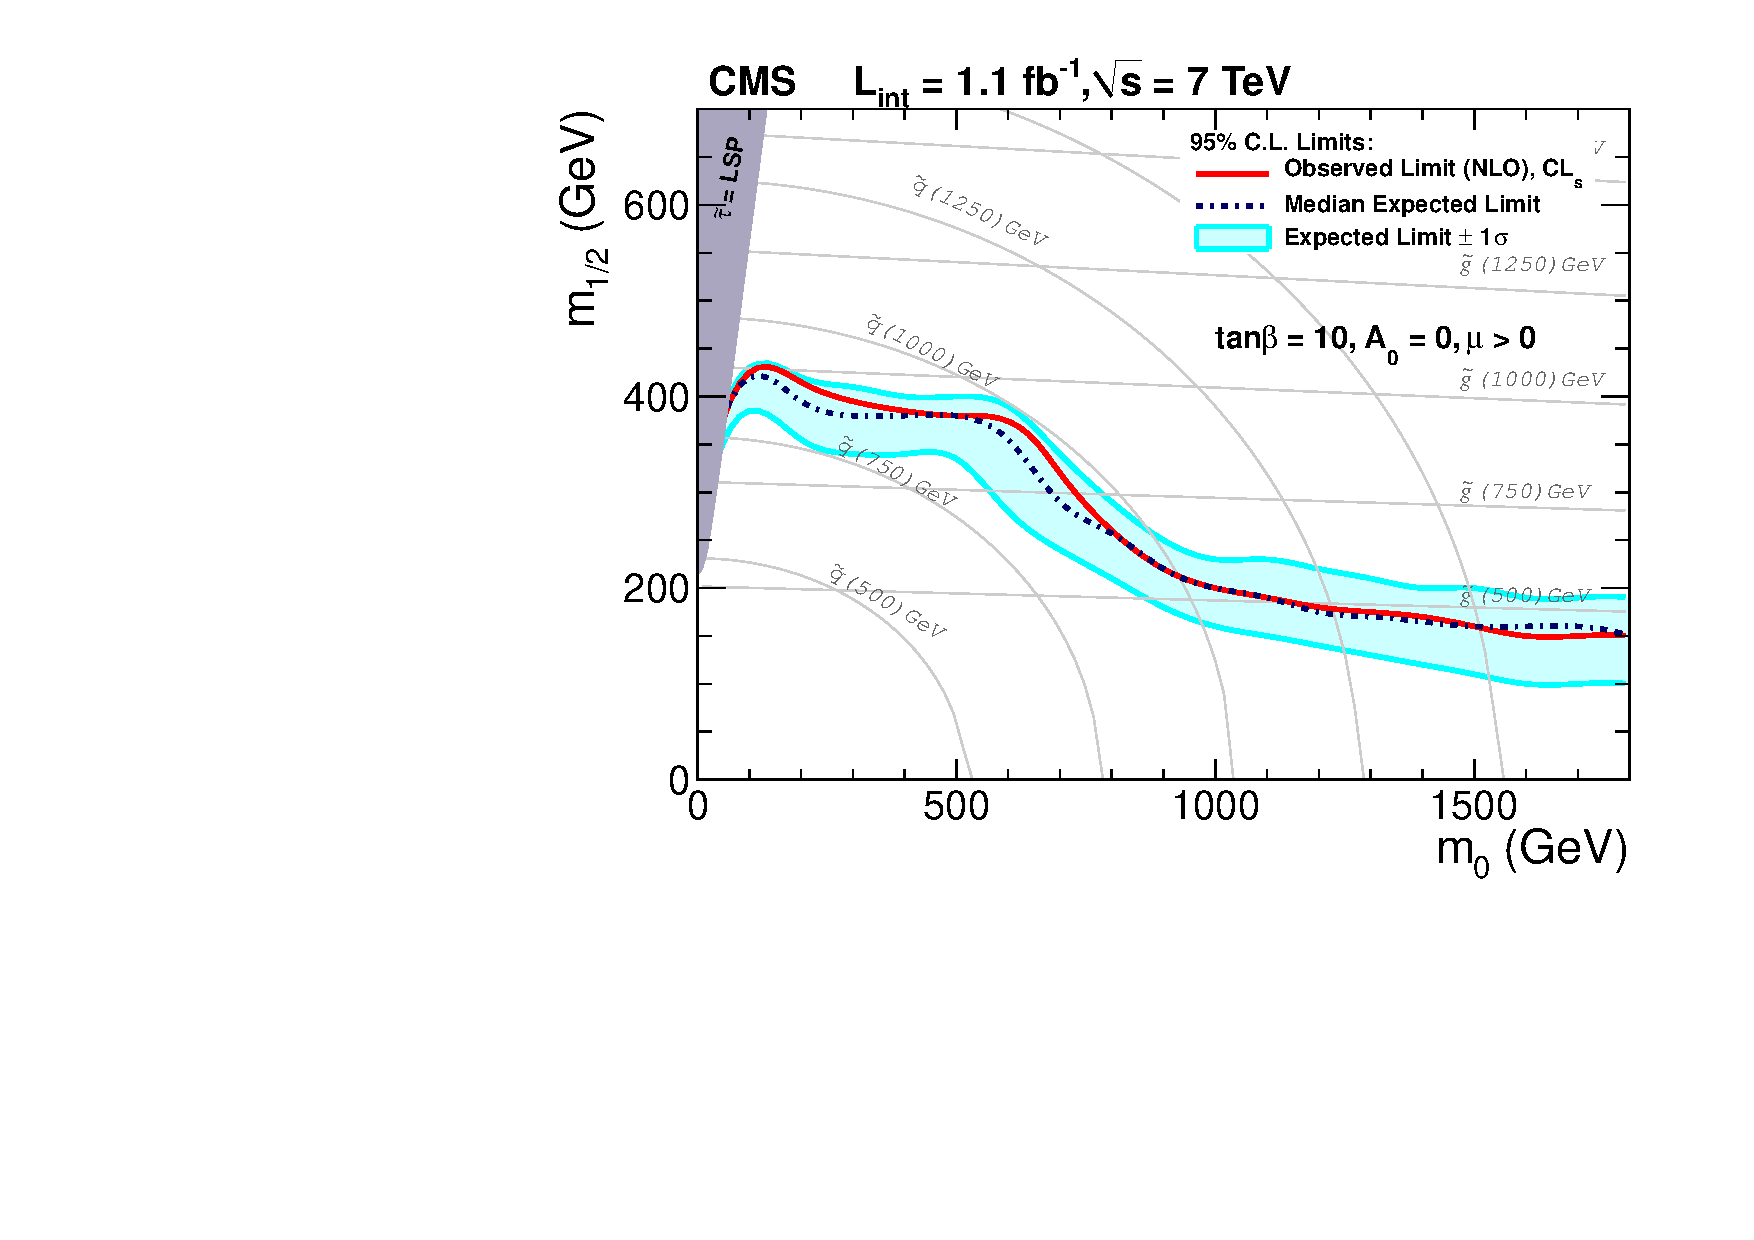
\includegraphics[width=\textwidth]{fig/RA4_ExclusionLimit_tanb10}
\caption[]{}
\label{fig:inter_msugra_exclusion}
\end{figure}

\subsection{\ac{T2tt}}
Similary the efficiency per \STlep bin with respect to the \ac{T2tt} parameter
space is shown in Figures~\ref{fig:inter_t2tt_mu} and \ref{fig:inter_t2tt_el}
respectively.
\begin{figure}
\centering
\subfloat[]{\label{fig:inter_t2tt_mu_eff250}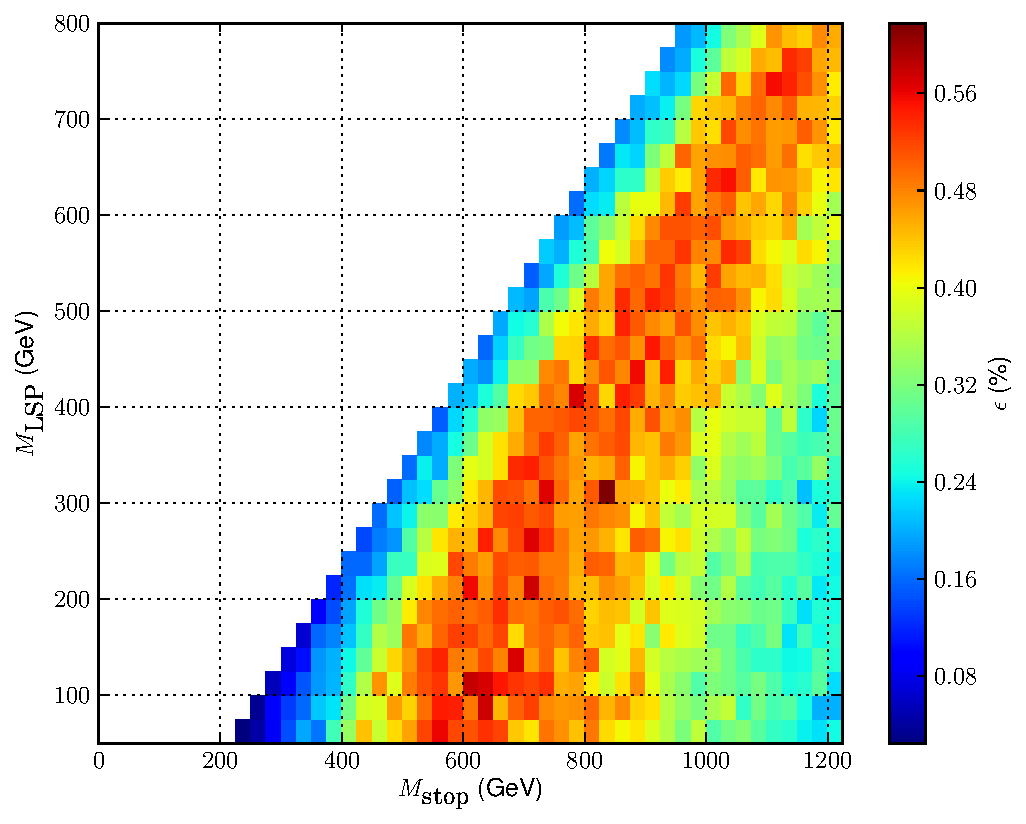
\includegraphics[width=0.49\textwidth]{fig/t2tt_muons_eff_250}}
\subfloat[]{\label{fig:inter_t2tt_mu_eff350}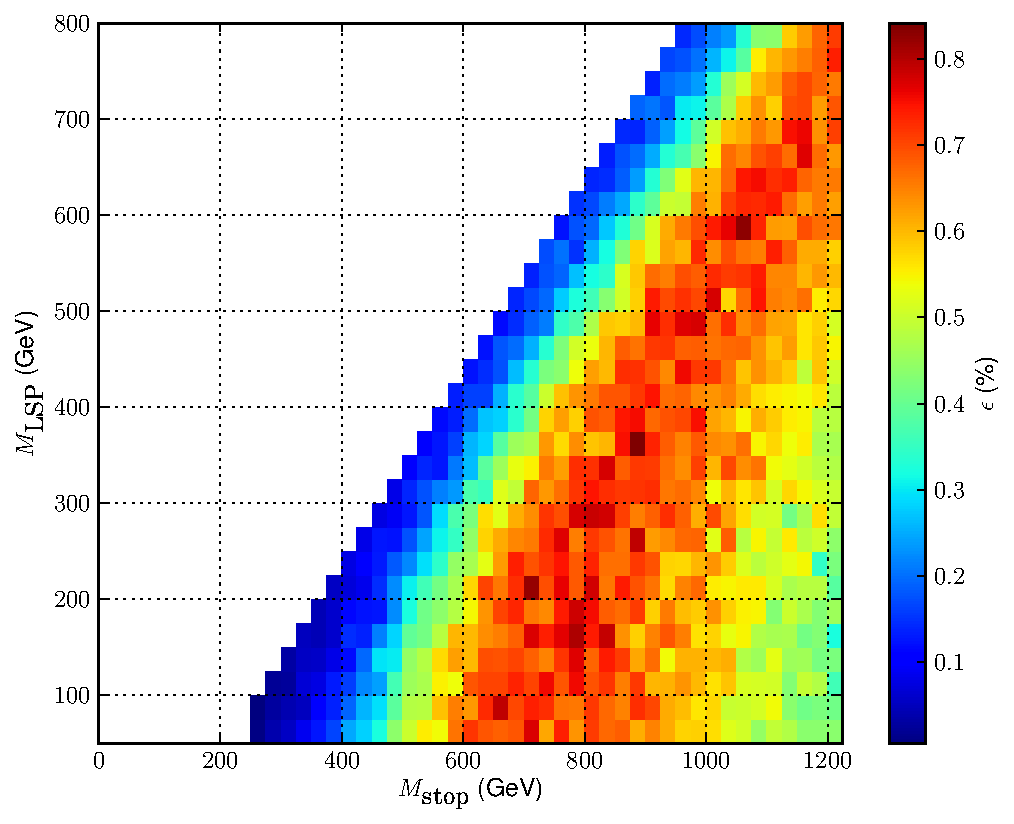
\includegraphics[width=0.49\textwidth]{fig/t2tt_muons_eff_350}}\\
\subfloat[]{\label{fig:inter_t2tt_mu_eff450}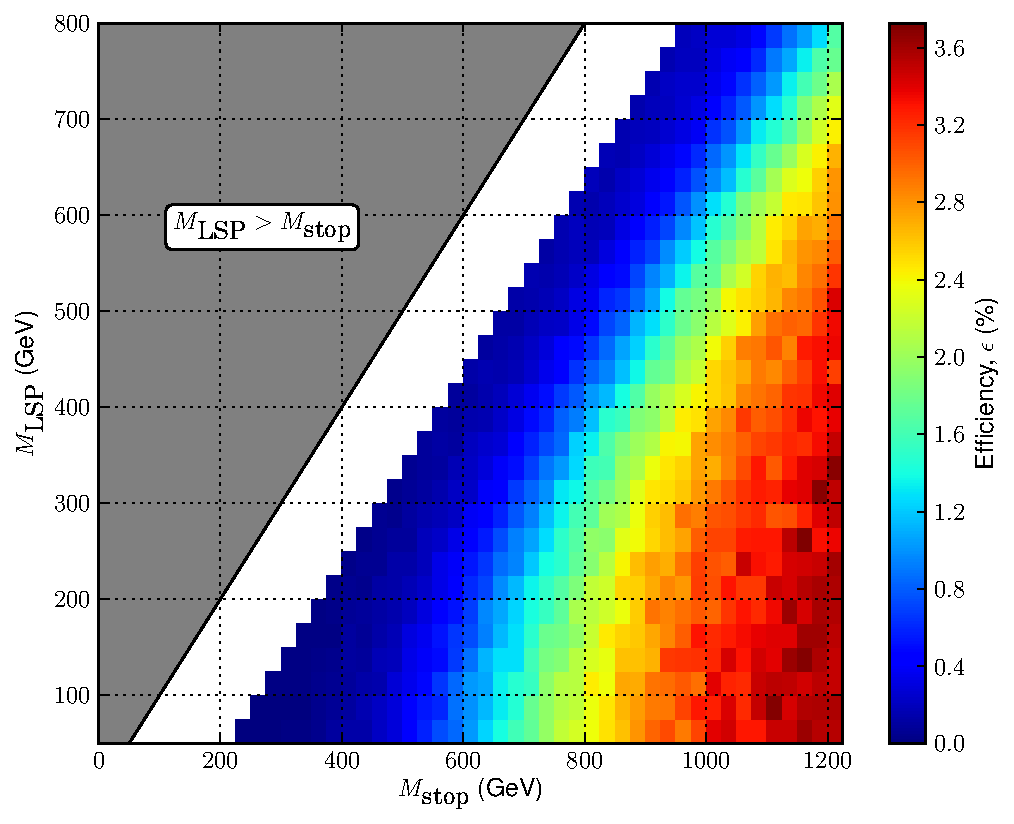
\includegraphics[width=0.49\textwidth]{fig/t2tt_muons_eff_450}}
\subfloat[]{\label{fig:inter_t2tt_mu_efftot}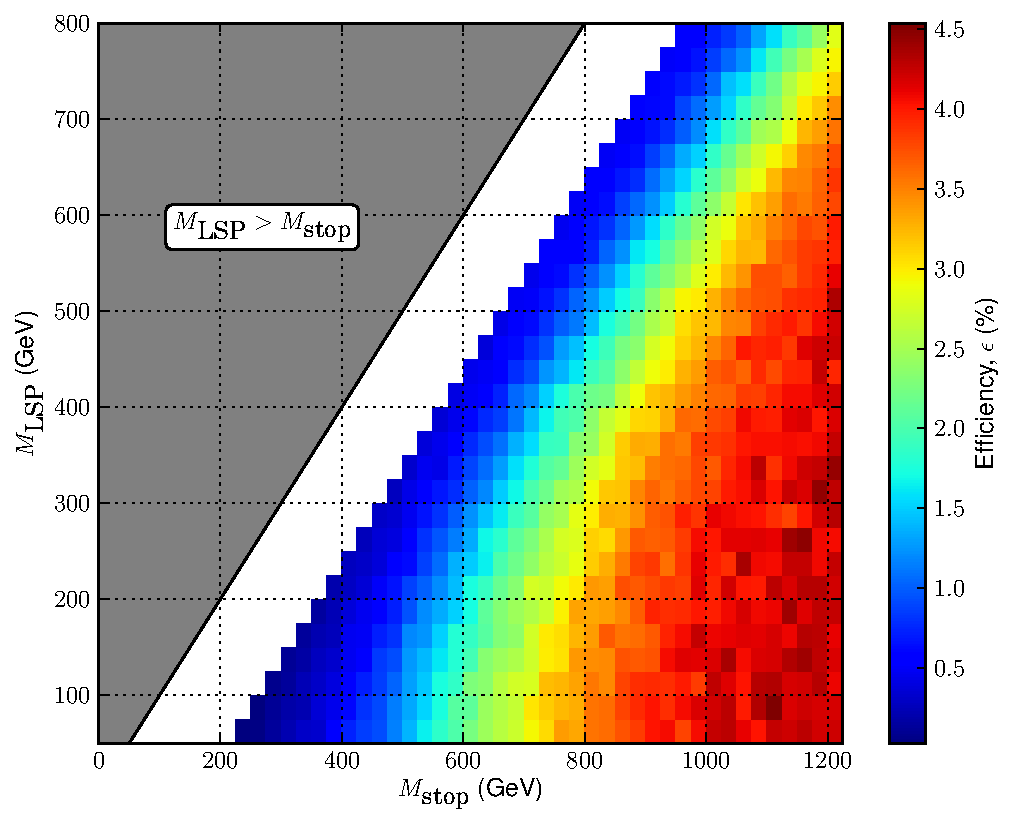
\includegraphics[width=0.49\textwidth]{fig/t2tt_muons_eff_total}}
\caption[]{}
\label{fig:inter_t2tt_mu}
\end{figure}

\begin{figure}
\centering
\subfloat[]{\label{fig:inter_t2tt_el_eff250}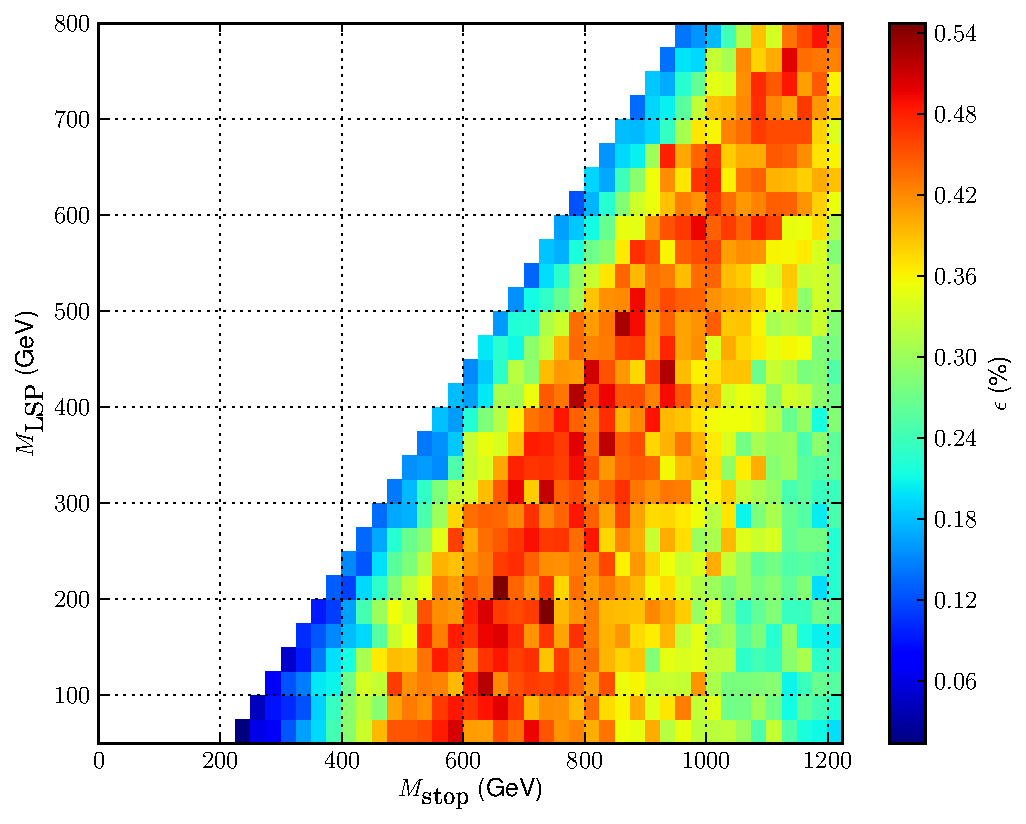
\includegraphics[width=0.49\textwidth]{fig/t2tt_electrons_eff_250}}
\subfloat[]{\label{fig:inter_t2tt_el_eff350}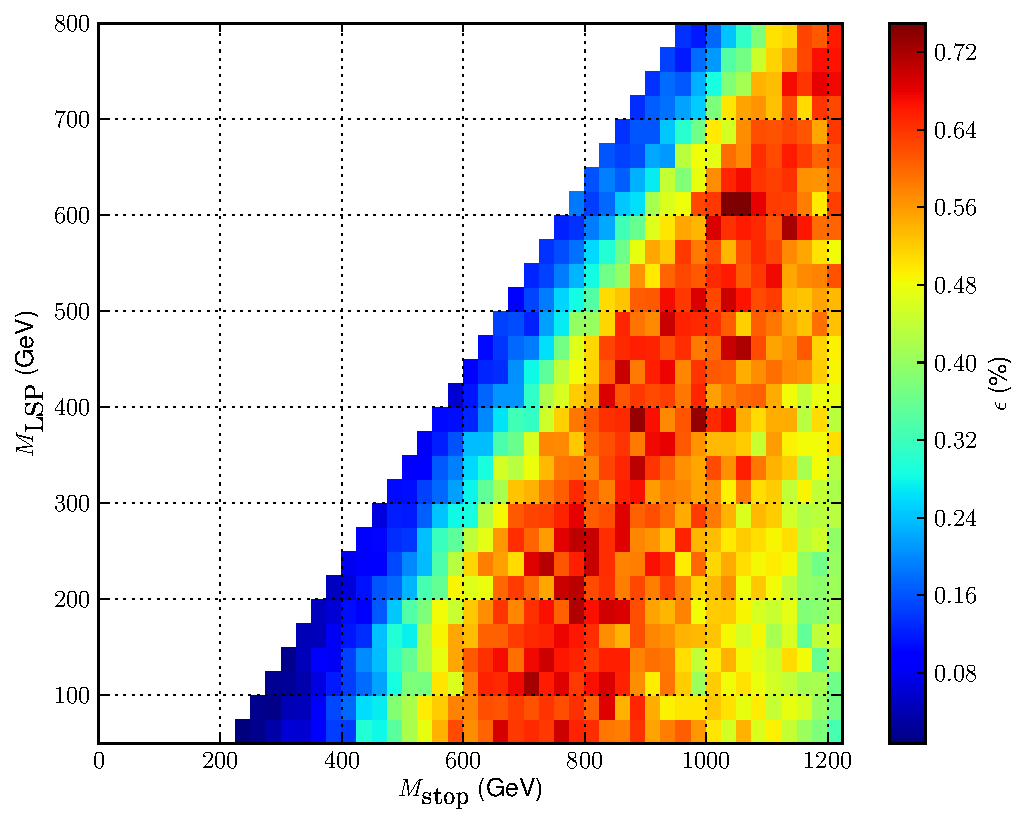
\includegraphics[width=0.49\textwidth]{fig/t2tt_electrons_eff_350}}\\
\subfloat[]{\label{fig:inter_t2tt_el_eff450}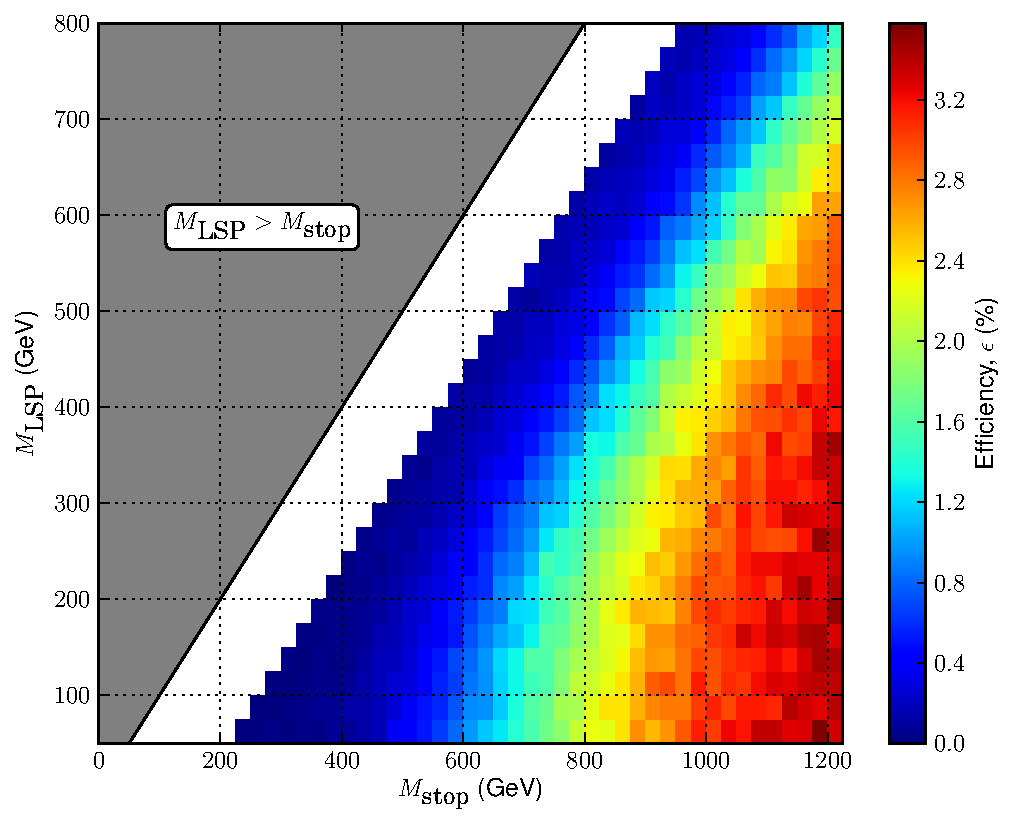
\includegraphics[width=0.49\textwidth]{fig/t2tt_electrons_eff_450}}
\subfloat[]{\label{fig:inter_t2tt_el_efftot}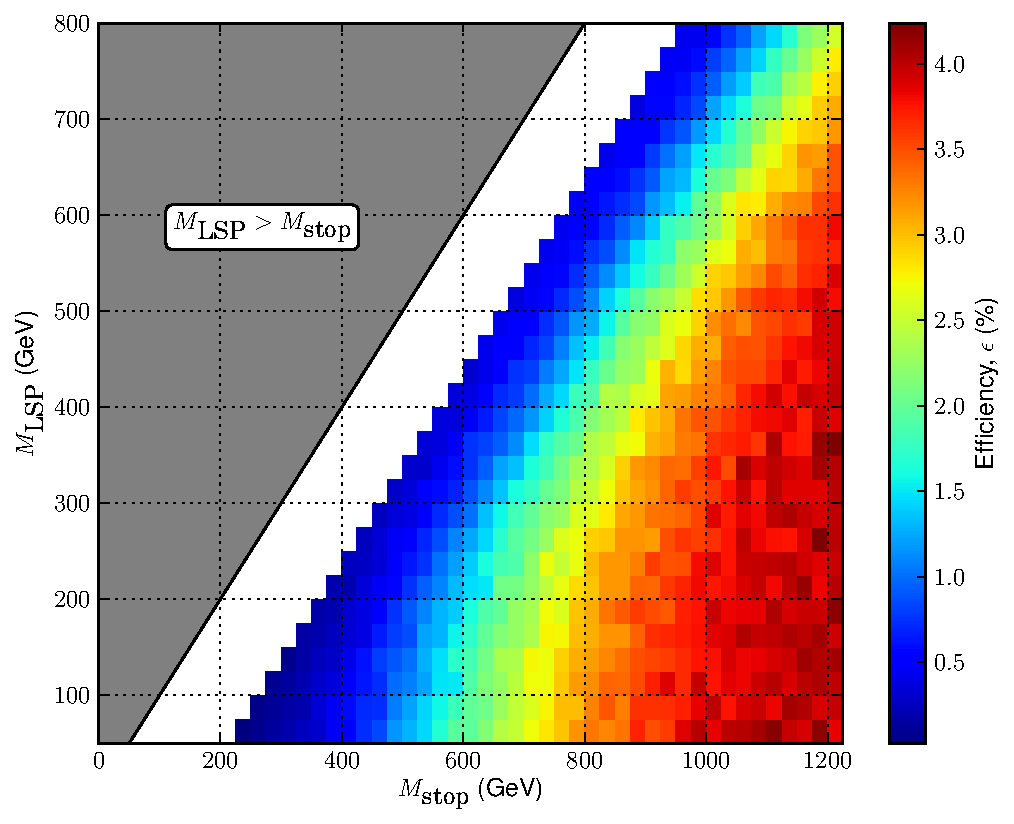
\includegraphics[width=0.49\textwidth]{fig/t2tt_electrons_eff_total}}
\caption[]{}
\label{fig:inter_t2tt_el}
\end{figure}


\begin{figure}
\centering
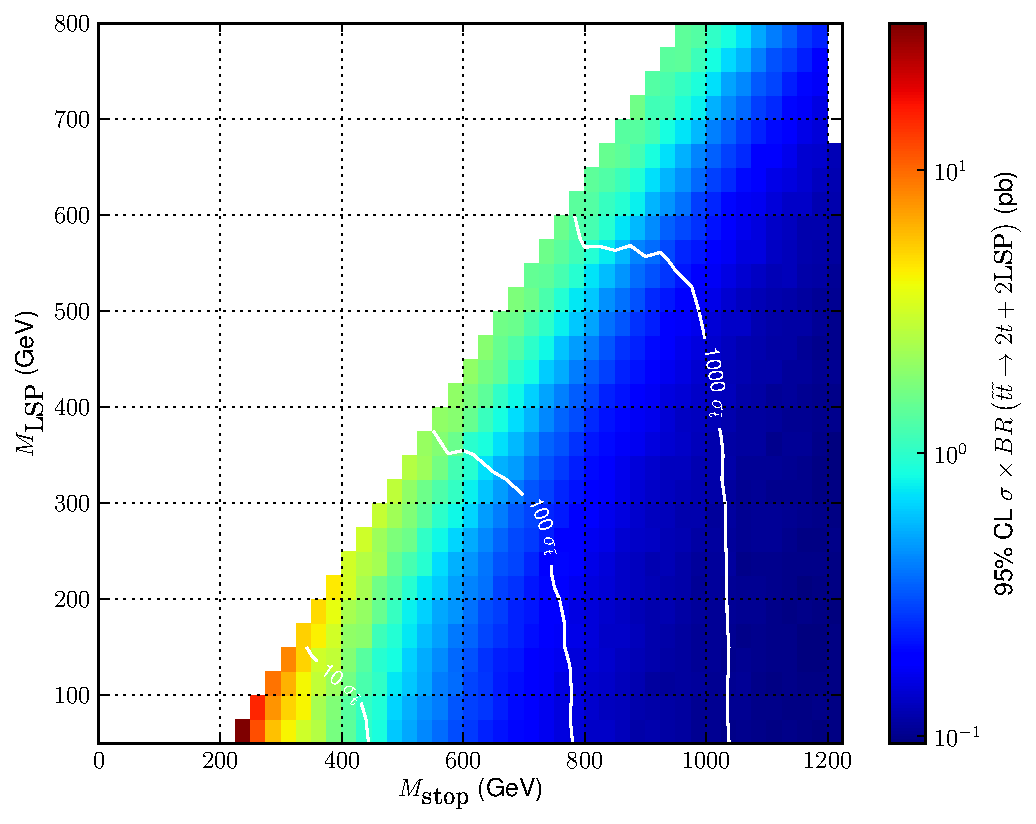
\includegraphics[width=0.49\textwidth]{fig/t2tt_limit}
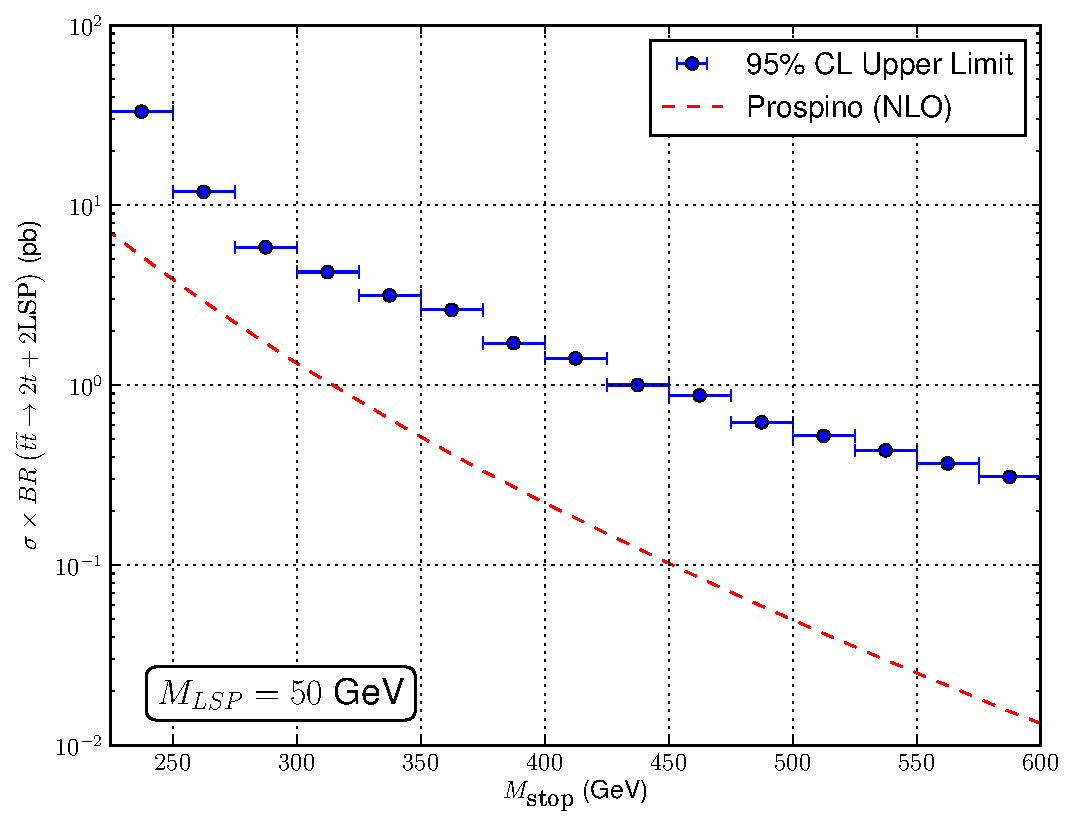
\includegraphics[width=0.49\textwidth]{fig/t2tt_limit_1d}
\caption[]{}
\label{fig:inter_t2tt}
\end{figure}

\begin{figure}

\end{figure}

%%% Local Variables:
%%% mode: latex
%%% TeX-master: "../thesis"
%%% End:
